
\chapter{Implementation in Isabelle}
\label{cha:implementation}

In this chapter we describe how the calculus of propositional dynamic logic has
been implemented in Isabelle. The implementation can roughly be divided into
three parts, which are first prerequisites like introducing the basic operations
of a monad and setting up a convenient syntax -- namely the do-notation -- for
compound monadic programs, second the definition or derivation of the logical
operators as well as several proof rules accompanying these, and third two
substantial example specifications from the realms of monadic parser combinators and
a classical while-program performing Russian multiplication.

To keep the notation within the main text and the inserted Isabelle example
specifications consistent, we will use the notation of Isabelle throughout this
chapter. One major change caused thereby is that we will write $\ivar{a} \Rightarrow
\ivar{b}\ T$ for the type of a polymorphic function which would otherwise be
denoted by $a \to T\ b$ (cf. \ref{sec:meta-basic-syntax}). Because the commonly
used symbols for the propositional connectives like $\land$ or $\longrightarrow$ are 
reserved for HOL, monadic connectives will be indexed by a $D$, as in $\land_D$
or $\longrightarrow_D$. Note also that implication is denoted by a simple arrow $\longrightarrow$ and not by
a double arrow $\Rightarrow$.
% An
% exception to this rule are the monadic propositional connectives, which have to
% be subscripted in Isabelle to differentiate them from the connectives of HOL. In
% the main text, however, these subscripts will be left out since the context will
% make clear whether, \EG, the conjunction $\land_D : \Type{bool}\ D \Rightarrow \Type{bool}\ D
% \Rightarrow \Type{bool}\ D$ of dynamic logic or the one of HOL $\land : \Type{bool} \Rightarrow
% \Type{bool} \Rightarrow \Type{bool}$ is under consideration.

\section{Theory Files}

The following listing of the theory files that have been created provides a more
detailed explanation of the overall structure of the implementation. Besides
that, Figure~\ref{fig:session-graph} shows the dependency graph of these
theories. In this diagram, a link between two theories indicates that the theory
below imports all theorems and definitions of the one above. In this way a simple
acyclic theory hierarchy can be created in Isabelle. The figure moreover
visualises the fact that the calculus directly builds on HOL, Isabelle's
formulation of higher-order logic. Theory \textit{Pure} is Isabelle's
meta-logic, hence the base theory for every other logic.

\begin{description}
\item[Monads] first of all defines a type constructor
  $T$ that takes values of type $\ivar{a}$ to monadic programs (or computations)
  of type $\ivar{a}\ T$.  Further it defines the monadic primitive operations
  $\bindOp$, $\seqOp$ and $\ret$ for binding, sequencing and creating monadic
  programs. Finally, a do-notation quite similar to the one found in Haskell is
  defined through Isabelle's syntax facility. \Eat{The implementation can be found on
  p.~\pageref{sec:monads-thy}ff.}

\item[MonProp] formalises the notions of discardability, copyability and
  deterministic side-effect freeness of monadic programs and the properties
  that these programs possess. The subtype $\ivar{a}\ D$ of dsef programs in
  $\ivar{a}\ T$ is introduced and operations $\op{liftM}, \op{liftM2}$, etc.,
  are defined allowing to lift HOL functions into the monadic setting. These
  will be used to define the propositional connectives. \Eat{$\Longrightarrow$
  p.~\pageref{sec:monprop-thy}ff.}

\item[MonLogic] constitutes the setup of the propositional part of monadic
  dynamic logic. It defines the propositional connectives in terms of the ones
  of HOL, enables the simplifier to solve propositional tautologies in the new
  logic automatically and proves `lifted' analogues of standard HOL rules like
  $\irule{conjI}$, $\irule{disjE}$ or $\irule{excluded-middle}$. \Eat{$\Longrightarrow$
  p.~\pageref{sec:monlogic-thy}ff. }

\item[PDL] completes the setup of the basic calculus by declaring the box and
  diamond operators, providing a convenient syntax for these, and formalising
  the proof calculus for dynamic logic of Section~\ref{sec:monad-indep-calc}.
  Additionally, it is shown how the classical relationship between the box and
  diamond operator is automatically established by basing the logic on HOL,
  which itself is classical. The theory file ends with several proof rules that
  are derived from the basic calculus. \Eat{$\Longrightarrow$ p.~\pageref{sec:pdl-thy}ff.}
  
\item[MonEq] is a rather short theory file adding equality to the set of lifted
  operations. Rules representing transitivity, reflexivity and symmetry of
  monadic equality are also given. \Eat{$\Longrightarrow$ p.~\pageref{sec:moneq-thy}ff.}

\item[Parsec] contains the axiomatisation of the basic operations of a monad for
  parser combinators in the style of \cite{HuttonMeijer96}. Subsequently, the
  specification and verification of a parser for natural numbers which is
  defined in terms of the basic parsers is presented. \Eat{$\Longrightarrow$
  p.~\pageref{sec:parsec-thy}ff. }

\item[State] specifies a monad with readable and writable references as well as
  a while loop. In this monad, the algorithm for Russian multiplication is
  specified and proved correct. \Eat{$\Longrightarrow$ p.~\pageref{sec:state-thy}ff.}

\end{description}

\begin{figure}
  \centering
  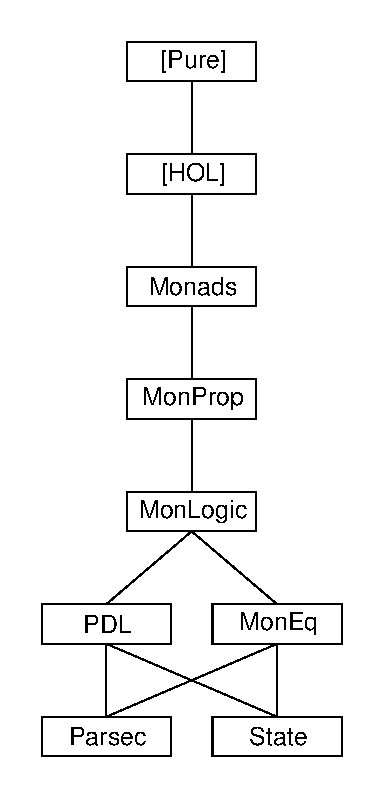
\includegraphics[width=0.35\textwidth]{session_graph}
  \caption{Dependency graph of the Isabelle theories}
  \label{fig:session-graph}
\end{figure}

\section{Monads in Isabelle}
\label{sec:monads-isabelle}
While in Haskell the common ground of all (computable) monads can at least be
captured at the level of operation types\footnote{which is done by making the
  respective type constructors like \texttt{[]} (being syntactical sugar for
  \texttt{List}), \texttt{Maybe}, etc., instances of the constructor class
  \texttt{Monad}}, Isabelle's concept of \emph{axiomatic type classes} is not
strong enough to suit this purpose.  Axiomatic type classes are like Haskell's
type classes, with the supplementary possibility of specifying what properties
the operations over a certain type class must satisfy. For example, the type
class $\Type{parord}$ of partial orders requires its instances to provide the
operations $<$ and $\leq$, but additionally demands that the latter satisfies the
usual properties of transitivity, reflexivity and antisymmetry. For the
specification of monads however one does not require a class of types but rather
a class of type constructors, namely the class of all those type constructors
mapping a given base type into the type of specific computations over this type.

Due to the lack of this concept our implementation simply declares a
polymorphic abstract type $\ivar{a}\ T$, where $T$ is supposed to stand for
the monad in question. This way of proceeding precludes the exact definition of
concrete monads and their primitive operations, since the structure of the monad
is not visible. From the viewpoint of Isabelle's \emph{definitional approach}
-- where HOL is supposed to be supplemented only by further definitions and
theorems rather than axioms -- this may be considered an imperfection, because
additional operations acting on the structure of the monad have to be described
axiomatically. For instance, there will be no way to define what precisely the
operations of writing to or reading a reference in the state monad do, but these
can only be described via their logical effects.  Nonetheless, the way
chosen here adheres to the one suggested in \cite{SchroederMossakowski:PDL} and,
in any case, the alternative would have been to have distinct base theories for
all concrete monads, which is hard to maintain and tedious to implement.

\begin{isabellebody}
\isanewline
\isamarkuptrue%
\isacommand{typedecl}\ {\isacharprime}a\ T\isanewline
\isanewline
\isamarkupfalse%
\isamarkuptrue%
\isacommand{consts}\isanewline
\ bind\ {\isacharcolon}{\isacharcolon}\ {\isachardoublequote}{\isacharprime}a\ T\ {\isasymRightarrow}\ {\isacharparenleft}{\isacharprime}a\ {\isasymRightarrow}\ {\isacharprime}b\ T{\isacharparenright}\ {\isasymRightarrow}\ {\isacharprime}b\ T{\isachardoublequote}\ \ \ \ \ {\isacharparenleft}\isakeyword{infixl}\ {\isachardoublequote}{\isasymggreater}{\isacharequal}{\isachardoublequote}\ {\isadigit{2}}{\isadigit{0}}{\isacharparenright}\isanewline
\ ret\ \ {\isacharcolon}{\isacharcolon}\ {\isachardoublequote}{\isacharprime}a\ {\isasymRightarrow}\ {\isacharprime}a\ T{\isachardoublequote}\isanewline
\isanewline
\isamarkupfalse%
\isacommand{constdefs}\isanewline
\ seq\ {\isacharcolon}{\isacharcolon}\ {\isachardoublequote}{\isacharprime}a\ T\ {\isasymRightarrow}\ {\isacharprime}b\ T\ {\isasymRightarrow}\ {\isacharprime}b\ T{\isachardoublequote}\ \ \ \ \ \ \ \ \ \ \ \ {\isacharparenleft}\isakeyword{infixl}\ {\isachardoublequote}{\isasymggreater}{\isachardoublequote}\ {\isadigit{2}}{\isadigit{0}}{\isacharparenright}\isanewline
\ {\isachardoublequote}p\ {\isasymggreater}\ q\ {\isasymequiv}\ {\isacharparenleft}p\ {\isasymggreater}{\isacharequal}\ {\isacharparenleft}{\isasymlambda}x{\isachardot}\ q{\isacharparenright}{\isacharparenright}{\isachardoublequote}\isamarkupfalse%
\isanewline%
\end{isabellebody}
This is the concrete Isabelle notation for the introduction of the type
$\ivar{a}\ T$ of monadic programs and the basic operations $\op{bind}$, $\ret$
and $\op{seq}$, where the latter is defined in terms of the binding. The
so-called \emph{mixfix annotations} on the right margin declare infix notation,
$\bindOp$ for $\op{bind}$ and $\seqOp$ for $\op{seq}$, which in their simple
form given here resemble the syntax annotations for infix operators in Haskell.
As stated above $\op{bind}$ and $\ret$ can only be declared as abstract
constants through a \textbf{consts} declaration, while $\op{seq}$ can be given a
declaration as well as a concrete definition (albeit in terms of the abstractly
defined operation $\op{bind}$, of course) through the \textbf{constdefs}
statement. The latter combines the effects of the statements \textbf{consts} and
\textbf{defs}, where the \textbf{defs} statement serves the purpose of providing
a definition for a previously introduced constant.

The following is a specification of the monad laws of Equation~(\ref{eq:mondef})
in Isabelle. The \emph{[simp]} instruction makes Isabelle hand a theorem
or axiom to the simplifier as a rewrite rule automatically. We have included a
specification that $\ret$ is injective. From these axioms
we can prove the associativity of $\seqOp$ immediately.
\begin{isabellebody}
\isanewline
\isamarkuptrue%
\isacommand{axioms}\isanewline
\ bind{\isacharunderscore}assoc\ {\isacharbrackleft}simp{\isacharbrackright}{\isacharcolon}\ {\isachardoublequote}{\isacharparenleft}p\ {\isasymggreater}{\isacharequal}\ {\isacharparenleft}{\isasymlambda}x{\isachardot}\ f\ x\ {\isasymggreater}{\isacharequal}\ g{\isacharparenright}{\isacharparenright}\ {\isacharequal}\ {\isacharparenleft}p\ {\isasymggreater}{\isacharequal}\ f\ {\isasymggreater}{\isacharequal}\ g{\isacharparenright}{\isachardoublequote}\isanewline
\ ret{\isacharunderscore}lunit\ {\isacharbrackleft}simp{\isacharbrackright}{\isacharcolon}\ {\isachardoublequote}{\isacharparenleft}ret\ x\ {\isasymggreater}{\isacharequal}\ f{\isacharparenright}\ {\isacharequal}\ f\ x{\isachardoublequote}\isanewline
\ ret{\isacharunderscore}runit\ {\isacharbrackleft}simp{\isacharbrackright}{\isacharcolon}\ {\isachardoublequote}{\isacharparenleft}p\ {\isasymggreater}{\isacharequal}\ ret{\isacharparenright}\ {\isacharequal}\ p{\isachardoublequote}\isanewline
\ ret{\isacharunderscore}inject{\isacharcolon}\ {\isachardoublequote}ret\ x\ {\isacharequal}\ ret\ z\ {\isasymLongrightarrow}\ x\ {\isacharequal}\ z{\isachardoublequote}\isanewline
\isanewline
\isamarkupfalse%
\isacommand{lemma}\ seq{\isacharunderscore}assoc\ {\isacharbrackleft}simp{\isacharbrackright}{\isacharcolon}\ {\isachardoublequote}{\isacharparenleft}p\ {\isasymggreater}\ {\isacharparenleft}q\ {\isasymggreater}\ r{\isacharparenright}{\isacharparenright}\ {\isacharequal}\ {\isacharparenleft}p\ {\isasymggreater}\ q\ {\isasymggreater}\ r{\isacharparenright}{\isachardoublequote}\isanewline
\ \isamarkupfalse%
\isacommand{by}\ {\isacharparenleft}simp\ add{\isacharcolon}\ seq{\isacharunderscore}def{\isacharparenright}\isamarkupfalse%
\isanewline%
\end{isabellebody}

\subsection{The do-Notation}
Next comes the setup of the do-notation by means of Isabelle's syntax
translation facility. This basically is a term-rewriting mechanism on abstract
syntax trees which can be configured by adding rewrite rules for either the
transformation of concrete input into a valid Isabelle term or vice versa. We
will not go into the details of this mechanism, which is laid out in the
Isabelle reference manual \cite{IsaRef04}. The implementation can be found in
Appendix~\ref{cha:isabelle-theories}, p.~\pageref{isa:do-notation}.

The syntax translations make it possible to write monadic programs in a much
more convenient way that mirrors the sequentiality inherent in these programs.
In the implementation we make use of this notation exclusively.  As an example,
one may write the following
\begin{align*}
& \DoStmt{x\leteq p; q\ x} && \DoStmt{x\leteq p; y\leteq q; r\ x\ y} &&
  \DoStmt{x\leteq p; y\leteq q; z\leteq r; \ret~(x,y,z)}\\
\intertext{instead of }
& p \bindOp \LambdaTerm{x}{q\ x}  && 
  p \bindOp (\LambdaTerm{x}{q\bindOp \LambdaTerm{y}{r\ x\ y}}) &&
  \DoStmt{x\leteq p;\DoStmt{y\leteq q; \DoStmt{z\leteq r; \ret~(x,y,z)}}}
\end{align*}
where the third column indicates that multiple
bindings may be input as a sequence rather than in a nested fashion. 
\begin{rem}
  The fact that do-terms are simply syntactical sugar also means that we do not
  formalise the inference rules of the meta-language for monads described in
  Section~\ref{sec:metalanguage-monads}, but rather work with monadic programs
  and their properties directly and just display them in the more convenient
  do-notation. That such a translation can be achieved purely by syntax
  transformations indicates how closely the meta-language is related to actual
  monadic programs.
\end{rem}


\subsection{Properties of Monadic Programs}
\label{sec:isa-prop-monad-progr}

Our main goal for now is to obtain a subtype $\ivar{a}\ D$ of deterministically
side effect free (\emph{dsef}) programs over $\ivar{a}\ T$ so that programs of
type $\Type{bool}\ D$ can be used as formulae of our logic. The kind of
subtyping supported by Isabelle proceeds by defining a new type in terms of a
subset of elements of an existing type. Isabelle then generates a bijection
between this subset of the existing type and the new type which consists of an
\emph{abstraction function} from the existing type into the new one -- which is
only sensibly defined for elements that really have a corresponding element in
the new type -- and a \emph{representation function} mapping elements of the
new type back to their representatives in the existing type. 

It is
straightforward to formalise the concepts of discardability and copyability, the
concepts on which the property $\op{dsef}$ builds. The latter is itself defined
in terms of the former ones as follows.

\begin{isabellebody}
\isamarkuptrue%
\isanewline
\isacommand{constdefs}\isanewline
\ \ dis\ {\isacharcolon}{\isacharcolon}\ {\isachardoublequote}{\isacharprime}a\ T\ {\isasymRightarrow}\ bool{\isachardoublequote}\isanewline
\ \ {\isachardoublequote}dis{\isacharparenleft}p{\isacharparenright}\ {\isasymequiv}\ {\isacharparenleft}do\ {\isacharbraceleft}x{\isasymleftarrow}p{\isacharsemicolon}\ ret{\isacharparenleft}{\isacharparenright}{\isacharbraceright}{\isacharparenright}\ {\isacharequal}\ ret\ {\isacharparenleft}{\isacharparenright}{\isachardoublequote}\isanewline
\isanewline
\ \ cp\ \ {\isacharcolon}{\isacharcolon}\ {\isachardoublequote}{\isacharprime}a\ T\ {\isasymRightarrow}\ bool{\isachardoublequote}\isanewline
\ \ {\isachardoublequote}cp{\isacharparenleft}p{\isacharparenright}\ {\isasymequiv}\ {\isacharparenleft}do\ {\isacharbraceleft}x{\isasymleftarrow}p{\isacharsemicolon}\ y{\isasymleftarrow}p{\isacharsemicolon}\ ret{\isacharparenleft}x{\isacharcomma}y{\isacharparenright}{\isacharbraceright}{\isacharparenright}\ {\isacharequal}\ {\isacharparenleft}do\ {\isacharbraceleft}x{\isasymleftarrow}p{\isacharsemicolon}\ ret{\isacharparenleft}x{\isacharcomma}x{\isacharparenright}{\isacharbraceright}{\isacharparenright}{\isachardoublequote}\isanewline
\isanewline
\ \ dsef\ {\isacharcolon}{\isacharcolon}\ {\isachardoublequote}{\isacharprime}a\ T\ {\isasymRightarrow}\ bool{\isachardoublequote}\isanewline
\ \ {\isachardoublequote}dsef{\isacharparenleft}p{\isacharparenright}\ {\isasymequiv}\ cp{\isacharparenleft}p{\isacharparenright}\ {\isasymand}\ dis{\isacharparenleft}p{\isacharparenright}\ {\isasymand}\ {\isacharparenleft}{\isasymforall}q{\isacharcolon}{\isacharcolon}bool\ T{\isachardot}\ cp{\isacharparenleft}q{\isacharparenright}\ {\isasymand}\ dis{\isacharparenleft}q{\isacharparenright}\ {\isasymlongrightarrow}\ \isanewline
\ \ \ \ \ \ \ \ \ \ \ \ \ \ \ \ \ \ \ \ \ \ \ \ \ \ \ \ \ \ \ \ \ \ \ \
cp{\isacharparenleft}do\
{\isacharbraceleft}x{\isasymleftarrow}p{\isacharsemicolon}\
y{\isasymleftarrow}q{\isacharsemicolon}\
ret{\isacharparenleft}x{\isacharcomma}y{\isacharparenright}{\isacharbraceright}{\isacharparenright}{\isacharparenright}{\isachardoublequote}\isanewline
\end{isabellebody}

The definition of $\op{dsef}$ deserves explanation for two reasons. First, it
should be repeated that there are three equivalent formulations of what it means
for a program to commute with some other program (cf. Def.~\ref{defn:commutes}),
from which we have chosen (\ref{eq:commutes-1}). Second, this formulation
restricts the types of programs that the given program $p$ has to commute with
to those of type $\Type{bool}$ (see also Definition~\ref{defn:dsef} and
Remark~\ref{rem:isa-type-restr}). This is required because Isabelle\footnote{to
  be precise, this statement is only true for logics like HOL which inherit
  their type mechanism from Isabelle's meta-logic} does not allow for a
quantification over type variables in a definition. But this is exactly what
would be done, if implicitly, in the case that the right-hand side of the
definition mentioned an arbitrary program $q :: \ivar{a}\ T$. As $\ivar{a}$
would be arbitrary, any type might serve as an instantiation. An explicit lemma
\irule{commute-bool-arb} is needed to derive the commutativity of a certain
program $p$ with copyable and discardable programs of \emph{any} type from the
commutativity of $p$ among copyable and discardable programs of type
$\Type{bool}$. Because the implementation of global dynamic judgements was the
subject of a different diploma thesis, this `lemma' is in fact provided as an
axiom in this thesis; given a more elaborate infrastructure, it would however be
provable.

Several properties of copyable and discardable programs discussed in
Section~\ref{sec:dl-prelim} have been formalised, the most frequently employed
of which are Lemmas~\ref{thm:dis-general} and \ref{thm:cp-general}
\begin{isabellebody}
\isanewline
\isamarkuptrue%
\isacommand{lemma}\ cp{\isacharunderscore}arb{\isacharcolon}\
{\isachardoublequote}cp\ p\ {\isasymLongrightarrow}\ do\
{\isacharbraceleft}x{\isasymleftarrow}p{\isacharsemicolon}\
y{\isasymleftarrow}p{\isacharsemicolon}\ r\ x\ y{\isacharbraceright}\
{\isacharequal}\ do\ {\isacharbraceleft}x{\isasymleftarrow}p{\isacharsemicolon}\
r\ x\ x{\isacharbraceright}{\isachardoublequote}\isanewline
\isacommand{lemma}\ dis{\isacharunderscore}left{\isacharcolon}\ {\isachardoublequote}dis{\isacharparenleft}p{\isacharparenright}\ {\isasymLongrightarrow}\ do\ {\isacharbraceleft}p{\isacharsemicolon}\ q{\isacharbraceright}\ {\isacharequal}\ q{\isachardoublequote}\isanewline
\isamarkupfalse%
\end{isabellebody}
\noindent Notice how the substitution of $x$ for $y$ in $r$ of lemma
\irule{cp-arb} is achieved by making $r$ a function of $x$ and $y$.
With the above definitions and lemmas at our disposal the type
$\ivar{a}\ D$ can be defined. 

\begin{isabellebody}
\isanewline
\isamarkuptrue%
\isacommand{typedef}\ {\isacharparenleft}Dsef{\isacharparenright}\ {\isacharparenleft}{\isacharprime}a{\isacharparenright}\ D\ {\isacharequal}\ {\isachardoublequote}{\isacharbraceleft}p{\isacharcolon}{\isacharcolon}{\isacharprime}a\ T{\isachardot}\ dsef\ p{\isacharbraceright}{\isachardoublequote}\isanewline
\ \ \isamarkupfalse%
\isacommand{apply}{\isacharparenleft}rule\ exI{\isacharbrackleft}of\ {\isacharunderscore}\ {\isachardoublequote}ret\ x{\isachardoublequote}{\isacharbrackright}{\isacharparenright}\isanewline
\ \ \isamarkupfalse%
\isacommand{apply}{\isacharparenleft}blast\ intro{\isacharcolon}\ dsef{\isacharunderscore}ret{\isacharparenright}\isanewline
\isamarkupfalse%
\isacommand{done}\isamarkupfalse%
\isanewline%
\end{isabellebody}

The proof obligation in the type definition arises due to the
restriction that types must not be empty. We use the program $\ret~x$ as a
witness, since stateless programs are always dsef. This fact has of course been
proved as lemma $\irule{dsef-ret}$ in Isabelle beforehand.
 The \textbf{typedef} statement declares the new
type $\ivar{a}\ D$ to be in bijective correspondence to the set $\op{Dsef}$ of
dsef programs in $\ivar{a}\ T$. The definition of this set is subsequently
available under the name $\irule{Dsef-def}$. What's more, two functions
$\ifun{Abs-Dsef} :: \ivar{a}\ T \Rightarrow \ivar{a}\ D$ and $\ifun{Rep-Dsef} :: \ivar{a}\
D \Rightarrow \ivar{a}\ T$ are generated that mediate between these two types. As the
functions may appear quite often in certain formulae, two abbreviations are
introduced: $\Uparrow p$ stands for $\ifun{Abs-Dsef}\ p$ and $\Downarrow P$ stands for
$\ifun{Rep-Dsef}\ P$. This is quite suggestive, in particular in those cases
where terms of the form $\Uparrow \Downarrow P$ or $\Downarrow \Uparrow p$ appear since one is visually reminded
that these operations cancel each other out.

\begin{rem} \label{rem:cast-ret-isabelle} The reason why terms of the form $\Uparrow p$
  will appear is that one may only write monadic programs in $T$, while
  the formulae of our logic live in $D$. This means that a compound
  truth-valued program $p = \DoStmt{x_1\leteq p_1; \cdots; x_n\leteq p_n; r\ x_1 \cdots
    x_n}$ that is dsef will nonetheless have type $\Type{bool}\ T$. This program
  has to be shifted to $\Type{bool}\ D$ to form the monadic formula $\Uparrow p$.
  Furthermore, there are several atomic programs -- with $\ret~x$ being the
  predominant one -- which are dsef and hence may appear in formulae when
  shifted. We initiate the convention of defining a formula $\op{Prog}
  \equiv\; \Uparrow \op{prog}$ for each atomic dsef program $\op{prog}$. Hence the shifted
  version of $\ret$ is $\op{Ret}:: \ivar{a} \Rightarrow \ivar{a}\ D$.
\end{rem}

Theory MonProp also contains proofs of characteristic properties of dsef
programs which are not shared by discardable or copyable programs. The two most
important facts are that neighbouring dsef programs may be swapped (Theorem
\irule{commute-dsef}, p.~\pageref{isa:commute-dsef}) and that dsef programs
are stable under sequential composition (Theorem \irule{dsef-seq},
p.~\pageref{isa:dsef-seq}). While the first one is quite immediate from the
definitions, the second one asks for a bit more work. 
\begin{isabellebody}
\isanewline
\isacommand{theorem}\ dsef{\isacharunderscore}seq{\isacharcolon}\ {\isachardoublequote}{\isasymlbrakk}dsef\ p{\isacharsemicolon}\ {\isasymforall}x{\isachardot}\ dsef\ {\isacharparenleft}q\ x{\isacharparenright}{\isasymrbrakk}\ {\isasymLongrightarrow}\ dsef\ {\isacharparenleft}do\ {\isacharbraceleft}x{\isasymleftarrow}p{\isacharsemicolon}\ q\ x{\isacharbraceright}{\isacharparenright}{\isachardoublequote}\isanewline
\end{isabellebody}

According to the definition of $\op{dsef}$ proving that $\DoStmt{x\leteq p; q\
  x}$ (call it $r$ in the following) is dsef amounts to showing three facts. The
first one is that $r$ is discardable. This follows from the fact that $p$ and
$q\ x$ are discardable for all $x$. The second one, namely that $r$ is copyable,
follows from the fact that $p$ and $q\ x$ commute with each other, so that the
defining equality of copyability holds for $r$ by the copyability of $p$ and $q\
x$. It must be noted here that while we used condition
(\ref{eq:commutes-1})\footnote{stating that the composition of two discardable
  and copyable programs is again copyable} as part of the defining property of
dsef programs, condition (\ref{eq:commutes-3})\footnote{which states the
  property of commutativity more instructively by actually swapping two
  programs} can easily be inferred from (\ref{eq:commutes-1}), a point that has
been shown in lemma \irule{commute-1-3}. The final fact to be shown is that
$r$ commutes with all copyable and discardable $\Type{bool}$-valued programs.
This follows similarly to the second fact, noting that $p$ and $q\ x$ alone
commute with all discardable and copyable $\Type{bool}$-valued programs.

\subsection{Equational Reasoning in Isar}
\label{sec:eq-reason-isar}
We will now shortly explain how Isar supports equational reasoning. As it is
used in this thesis, equational reasoning means reasoning by chains of
equations, where each separate step is justified mainly by substituting equals
for equals. Take the following lemma, representing the formalisation of how to
infer (\ref{eq:commutes-2}) from (\ref{eq:commutes-1}), as an example.

\begin{isabellebody}
\isanewline
\isacommand{lemma}\ commute{\isacharunderscore}{\isadigit{1}}{\isacharunderscore}{\isadigit{2}}{\isacharcolon}\ {\isachardoublequote}{\isasymlbrakk}cp\ q{\isacharsemicolon}\ cp\ p{\isacharsemicolon}\ dis\ q{\isacharsemicolon}\ dis\ p{\isasymrbrakk}\ {\isasymLongrightarrow}\ cp\ {\isacharparenleft}do\ {\isacharbraceleft}x{\isasymleftarrow}p{\isacharsemicolon}\ y{\isasymleftarrow}q{\isacharsemicolon}\ ret{\isacharparenleft}x{\isacharcomma}y{\isacharparenright}{\isacharbraceright}{\isacharparenright}\isanewline
\ \ \ \ \ \ \ \ \ \ \ \ \ \ \ \ \ \ \ \ {\isasymLongrightarrow}\ do\ {\isacharbraceleft}x{\isasymleftarrow}p{\isacharsemicolon}\ y{\isasymleftarrow}q{\isacharsemicolon}\ ret{\isacharparenleft}x{\isacharcomma}y{\isacharparenright}{\isacharbraceright}\ {\isacharequal}\ do\ {\isacharbraceleft}y{\isasymleftarrow}q{\isacharsemicolon}\ x{\isasymleftarrow}p{\isacharsemicolon}\ ret{\isacharparenleft}x{\isacharcomma}y{\isacharparenright}{\isacharbraceright}{\isachardoublequote}\isanewline
\isamarkupfalse%
\isacommand{proof}\ {\isacharminus}\isanewline
\ \ \isamarkupfalse%
\isacommand{assume}\ a{\isacharcolon}\ {\isachardoublequote}cp\ q{\isachardoublequote}\ {\isachardoublequote}cp\ p{\isachardoublequote}\ {\isachardoublequote}dis\ q{\isachardoublequote}\ {\isachardoublequote}dis\ p{\isachardoublequote}\isanewline
\ \ \isamarkupfalse%
\isacommand{assume}\ c{\isacharcolon}\ {\isachardoublequote}cp\ {\isacharparenleft}do\ {\isacharbraceleft}x{\isasymleftarrow}p{\isacharsemicolon}\ y{\isasymleftarrow}q{\isacharsemicolon}\ ret{\isacharparenleft}x{\isacharcomma}y{\isacharparenright}{\isacharbraceright}{\isacharparenright}{\isachardoublequote}\isanewline
\ \ \isamarkupfalse%
\isacommand{let}\ {\isacharquery}s\ {\isacharequal}\ {\isachardoublequote}do\ {\isacharbraceleft}x{\isasymleftarrow}p{\isacharsemicolon}\ y{\isasymleftarrow}q{\isacharsemicolon}\ ret{\isacharparenleft}x{\isacharcomma}y{\isacharparenright}{\isacharbraceright}{\isachardoublequote}\isanewline
\ \ \isamarkupfalse%
\isacommand{have}\ {\isachardoublequote}{\isacharquery}s\ {\isacharequal}\ do\ {\isacharbraceleft}z{\isasymleftarrow}{\isacharquery}s{\isacharsemicolon}\ ret\ {\isacharparenleft}fst\ z{\isacharcomma}\ snd\ z{\isacharparenright}{\isacharbraceright}{\isachardoublequote}\ \isamarkupfalse%
\isacommand{by}\ simp\isanewline
\ \ \isamarkupfalse%
\isacommand{also}\ \isamarkupfalse%
\isacommand{from}\ c\ \isamarkupfalse%
\isacommand{have}\ {\isachardoublequote}{\isasymdots}\ {\isacharequal}\ do\ {\isacharbraceleft}w{\isasymleftarrow}{\isacharquery}s{\isacharsemicolon}\ z{\isasymleftarrow}{\isacharquery}s{\isacharsemicolon}\ ret\ {\isacharparenleft}fst\ z{\isacharcomma}\ snd\ w{\isacharparenright}{\isacharbraceright}{\isachardoublequote}\ \isamarkupfalse%
\isacommand{by}\ {\isacharparenleft}simp\ add{\isacharcolon}\ cp{\isacharunderscore}arb{\isacharparenright}\isanewline
\ \ \isamarkupfalse%
\isacommand{also}\ \isamarkupfalse%
\isacommand{from}\ a\ \isamarkupfalse%
\isacommand{have}\ {\isachardoublequote}{\isasymdots}\ {\isacharequal}\ do\ {\isacharbraceleft}v{\isasymleftarrow}q{\isacharsemicolon}\ x{\isasymleftarrow}p{\isacharsemicolon}\ ret{\isacharparenleft}x{\isacharcomma}v{\isacharparenright}{\isacharbraceright}{\isachardoublequote}\ \isamarkupfalse%
\isacommand{by}\ {\isacharparenleft}simp\ add{\isacharcolon}\ mon{\isacharunderscore}ctr\ dis{\isacharunderscore}left{\isadigit{2}}{\isacharparenright}\isanewline
\ \ \isamarkupfalse%
\isacommand{finally}\ \isamarkupfalse%
\isacommand{show}\ {\isacharquery}thesis\ \isamarkupfalse%
\isacommand{{\isachardot}}\isanewline
\isamarkupfalse%
\isacommand{qed}\isamarkupfalse%
\isanewline
\end{isabellebody}

\noindent After stating the valid assumptions and setting $?s$ as an
abbreviation for the left-hand side of the equation that is to be shown, a chain
of equations starts beginning with $?s$ and ending with the right-hand side of
the main goal. This kind of successive equational reasoning is realised in Isar
through a sequence of \textbf{have}\ldots \textbf{also have}\ldots statements and a
concluding \textbf{finally} statement. In its simplest form, the \textbf{also}
statement combines two facts of the form $a = b$ and $b = c$ to yield the fact
$a = c$, thus simply exploiting transitivity of equality. The \textbf{finally}
statement reiterates the transitive chain build up so far and feeds it into the
concluding proof -- which in the example is precisely the goal thesis. As a
convenience, three dots `\ldots' within a term refer to the right-hand side of the
most recently established equality. The main workhorse for performing the
intermediate proof steps is the simplifier, since it is ideally suited for
handling equalities and substitution. \cite{BauerWenzel01} contains a detailed
description of extended features of this mechanism, showing how it can also be
applied to  inequalities.


\subsection{Lifting HOL Constants}
\label{sec:lift-hol-const}


The definition of the propositional connectives in Section~\ref{sec:prim-conn}
suggests the introduction of \emph{lifting operators} that allow one to embed
HOL operators into the monadic setting. These lifting operators are well known
from Haskell and their definition in Isabelle does not look that different. The
basic idea is that to apply an $n$-ary operator $f :: [a_1,\ldots,a_n]
\Rightarrow b$ to $n$ monadic programs $p_1 :: a_1\,T, \ldots,  p_n::a_n\,T$, one
simply evaluates these programs in turn and applies the operator to the results.
In principle all HOL operators like equality, comparisons, addition, etc. could
be lifted this way, but for simplicity we will only lift the propositional
connectives and equality in the sequel.

\begin{isabellebody}
\isanewline
\isacommand{constdefs}\isanewline
\ liftM\ {\isacharcolon}{\isacharcolon}\ {\isachardoublequote}{\isacharbrackleft}{\isacharprime}a\ {\isasymRightarrow}\ {\isacharprime}b{\isacharcomma}\ {\isacharprime}a\ T{\isacharbrackright}\ {\isasymRightarrow}\ {\isacharprime}b\ T{\isachardoublequote}\isanewline
\ {\isachardoublequote}liftM\ f\ p\ {\isasymequiv}\ do\ {\isacharbraceleft}x\ {\isasymleftarrow}\ p{\isacharsemicolon}\ ret\ {\isacharparenleft}f\ x{\isacharparenright}{\isacharbraceright}{\isachardoublequote}\isanewline
\ liftM{\isadigit{2}}\ {\isacharcolon}{\isacharcolon}\ {\isachardoublequote}{\isacharbrackleft}{\isacharprime}a\ {\isasymRightarrow}\ {\isacharprime}b\ {\isasymRightarrow}\ {\isacharprime}c{\isacharcomma}\ {\isacharprime}a\ T{\isacharcomma}\ {\isacharprime}b\ T{\isacharbrackright}\ {\isasymRightarrow}\ {\isacharprime}c\ T{\isachardoublequote}\isanewline
\ {\isachardoublequote}liftM{\isadigit{2}}\ f\ p\ q\ {\isasymequiv}\ do\ {\isacharbraceleft}x\ {\isasymleftarrow}\ p{\isacharsemicolon}\ y\ {\isasymleftarrow}\ q{\isacharsemicolon}\ ret\ {\isacharparenleft}f\ x\ y{\isacharparenright}{\isacharbraceright}{\isachardoublequote}\isanewline
\end{isabellebody}

Thanks to lemma \irule{dsef-seq} it is very easy to prove that applying a
lifted operation to dsef programs yields a dsef program:
\begin{isabellebody}
\isanewline
\isacommand{lemma}\ dsef{\isacharunderscore}liftM{\isadigit{2}}{\isacharcolon}\
{\isachardoublequote}{\isasymlbrakk}dsef\ p{\isacharsemicolon}\ dsef\
q{\isasymrbrakk}\ {\isasymLongrightarrow}\ dsef\
{\isacharparenleft}liftM{\isadigit{2}}\ f\ p\
q{\isacharparenright}{\isachardoublequote}\isanewline
\end{isabellebody}
\noindent This fact is essential when introducing the propositional connectives
in this manner, since \EG the conjunction of two formulae is of course required
to be a formula, hence dsef.

\section{Setting up the Logic}
\label{sec:setting-up-logic}

Apart from a slight visual clutter induced by the occurrences of the shifting
functions $\Uparrow$ and $\Downarrow$ the definition of global validity (which we denote here by
a turnstile $\vdash$ instead of the global box $\gbox$) and of the propositional
connectives is now straightforward. We take conjunction, disjunction and
implication as primitives: the constant for falsity does not have do be defined,
since it is available via the injection of $\op{False}$ into the monad, \IE via
$\Ret~\op{False}$.
\begin{isabellebody}
\isanewline
\isacommand{consts}\isanewline
\ {\isachardoublequote}Valid{\isachardoublequote}\ \ \ \ \ \ \ {\isacharcolon}{\isacharcolon}\ {\isachardoublequote}bool\ D\ {\isasymRightarrow}\ bool{\isachardoublequote}\ \ \ \ \ \ \ \ \ \ \ \ \ \ \ {\isacharparenleft}{\isachardoublequote}{\isacharparenleft}{\isasymturnstile}\ {\isacharunderscore}{\isacharparenright}{\isachardoublequote}\ {\isadigit{1}}{\isadigit{5}}{\isacharparenright}\isanewline
\ {\isachardoublequote}{\isasymand}\isactrlsub D{\isachardoublequote}\ \ \ \ \ \ \ \ \ {\isacharcolon}{\isacharcolon}\ {\isachardoublequote}{\isacharbrackleft}bool\ D{\isacharcomma}\ bool\ D{\isacharbrackright}\ {\isasymRightarrow}\ bool\ D{\isachardoublequote}\ \ \ \ \ {\isacharparenleft}\isakeyword{infixr}\ {\isadigit{3}}{\isadigit{5}}{\isacharparenright}\isanewline
\ {\isachardoublequote}{\isasymor}\isactrlsub D{\isachardoublequote}\ \ \ \ \ \ \ \ \ {\isacharcolon}{\isacharcolon}\ {\isachardoublequote}{\isacharbrackleft}bool\ D{\isacharcomma}\ bool\ D{\isacharbrackright}\ {\isasymRightarrow}\ bool\ D{\isachardoublequote}\ \ \ \ \ {\isacharparenleft}\isakeyword{infixr}\ {\isadigit{3}}{\isadigit{0}}{\isacharparenright}\isanewline
\ {\isachardoublequote}{\isasymlongrightarrow}\isactrlsub D{\isachardoublequote}\ \ \ \ \ \ \ \ {\isacharcolon}{\isacharcolon}\ {\isachardoublequote}{\isacharbrackleft}bool\ D{\isacharcomma}\ bool\ D{\isacharbrackright}\ {\isasymRightarrow}\ bool\ D{\isachardoublequote}\ \ \ \ {\isacharparenleft}\isakeyword{infixr}\ {\isadigit{2}}{\isadigit{5}}{\isacharparenright}\isamarkupfalse%
\isanewline
\isacommand{defs}\isanewline
\ \ Valid{\isacharunderscore}def{\isacharcolon}\ {\isachardoublequote}{\isasymturnstile}\ P\ {\isasymequiv}\ {\isasymDown}\ P\ {\isacharequal}\ do\ {\isacharbraceleft}x{\isasymleftarrow}{\isacharparenleft}{\isasymDown}\ P{\isacharparenright}{\isacharsemicolon}\ ret\ True{\isacharbraceright}{\isachardoublequote}\isanewline
\ \ conjD{\isacharunderscore}def{\isacharcolon}\ {\isachardoublequote}P\ {\isasymand}\isactrlsub D\ Q\ {\isasymequiv}\ {\isasymUp}\ {\isacharparenleft}liftM{\isadigit{2}}\ {\isacharparenleft}op\ {\isasymand}{\isacharparenright}\ {\isacharparenleft}{\isasymDown}\ P{\isacharparenright}\ {\isacharparenleft}{\isasymDown}\ Q{\isacharparenright}{\isacharparenright}{\isachardoublequote}\isanewline
\ \ disjD{\isacharunderscore}def{\isacharcolon}\ {\isachardoublequote}P\ {\isasymor}\isactrlsub D\ Q\ {\isasymequiv}\ {\isasymUp}\ {\isacharparenleft}liftM{\isadigit{2}}\ {\isacharparenleft}op\ {\isasymor}{\isacharparenright}\ {\isacharparenleft}{\isasymDown}\ P{\isacharparenright}\ {\isacharparenleft}{\isasymDown}\ Q{\isacharparenright}{\isacharparenright}{\isachardoublequote}\isanewline
\ \ impD{\isacharunderscore}def{\isacharcolon}\ \ {\isachardoublequote}P\ {\isasymlongrightarrow}\isactrlsub D\ Q\ {\isasymequiv}\ {\isasymUp}\ {\isacharparenleft}liftM{\isadigit{2}}\ {\isacharparenleft}op\ {\isasymlongrightarrow}{\isacharparenright}\ {\isacharparenleft}{\isasymDown}\ P{\isacharparenright}\ {\isacharparenleft}{\isasymDown}\ Q{\isacharparenright}{\isacharparenright}{\isachardoublequote}\isanewline
\end{isabellebody}
Other operators like equivalence $\longleftrightarrow$ and negation
$\lnot$ are defined as abbreviations in the usual way:
\begin{isabellebody}
\isanewline
\isacommand{constdefs}\isanewline
\ iffD\ \ \ \ \ \ \ \ {\isacharcolon}{\isacharcolon}\ {\isachardoublequote}{\isacharbrackleft}bool\ D{\isacharcomma}\ bool\ D{\isacharbrackright}\ {\isasymRightarrow}\ bool\ D{\isachardoublequote}\ \ \ {\isacharparenleft}\isakeyword{infixr}\ {\isachardoublequote}{\isasymlongleftrightarrow}\isactrlsub D{\isachardoublequote}\ {\isadigit{2}}{\isadigit{0}}{\isacharparenright}\isanewline
\ {\isachardoublequote}P\ {\isasymlongleftrightarrow}\isactrlsub D\ Q\ {\isasymequiv}\ {\isacharparenleft}P\ {\isasymlongrightarrow}\isactrlsub D\ Q{\isacharparenright}\ {\isasymand}\isactrlsub D\ {\isacharparenleft}Q\ {\isasymlongrightarrow}\isactrlsub D\ P{\isacharparenright}{\isachardoublequote}\isanewline
\ NotD\ \ \ \ \ \ \ \ {\isacharcolon}{\isacharcolon}\ {\isachardoublequote}bool\ D\ {\isasymRightarrow}\ bool\ D{\isachardoublequote}\ \ \ \ \ \ \ \ \ \ \ \ \ \ {\isacharparenleft}{\isachardoublequote}{\isasymnot}\isactrlsub D\ {\isacharunderscore}{\isachardoublequote}\ {\isacharbrackleft}{\isadigit{4}}{\isadigit{0}}{\isacharbrackright}\ {\isadigit{4}}{\isadigit{0}}{\isacharparenright}\isanewline
\ \ {\isachardoublequote}{\isasymnot}\isactrlsub D\ P\ {\isasymequiv}\ P\ {\isasymlongrightarrow}\isactrlsub D\ Ret\ False{\isachardoublequote}\isamarkupfalse%
\isanewline
\end{isabellebody}
The notion of global validity can be simplified, since dsef programs are
discardable. This fact can be stated either as an equality in $T$ or as an
equality in $D$:
\begin{isabellebody}
  \isanewline
  \isacommand{lemma}\ Valid{\isacharunderscore}simp{\isacharcolon}\
  {\isachardoublequote}{\isacharparenleft}{\isasymturnstile}\
  p{\isacharparenright}\ {\isacharequal}\ {\isacharparenleft}{\isasymDown}\ p\
  {\isacharequal}\ ret\ True{\isacharparenright}{\isachardoublequote}\isanewline
  \isacommand{lemma}\ Valid{\isacharunderscore}simpD{\isacharcolon}\ {\isachardoublequote}{\isacharparenleft}{\isasymturnstile}\ P{\isacharparenright}\ {\isacharequal}\ {\isacharparenleft}P\ {\isacharequal}\ Ret\ True{\isacharparenright}{\isachardoublequote}\isanewline
\end{isabellebody}

\begin{rem}
  While the formalisation of the proof calculus as given in
  \cite{SchroederMossakowski:PDL} is tailored towards an intuitionistic
  framework, an immediate consequence of the definitions presented thus far is
  that \emph{the implementation of the calculus in Isabelle is classical}. This
  follows from the fact that the logical operators are defined in terms of the
  HOL operators and that $\Type{bool}$ is classical, \IE contains only two
  values $\op{True}$ and $\op{False}$. A representative theorem confirming that a
  logic is classical is the law of excluded middle. The formulation in the
  monadic setting reads as
  \begin{isabellebody} \isanewline
    \isacommand{theorem}\ pdl{\isacharunderscore}excluded{\isacharunderscore}middle{\isacharcolon}\ {\isachardoublequote}{\isasymturnstile}\ P\ {\isasymor}\isactrlsub D\ {\isacharparenleft}{\isasymnot}\isactrlsub D\ P{\isacharparenright}{\isachardoublequote}\isanewline
  \end{isabellebody}
  The outline of the proof of this theorem is as follows: first, decode $P \lor_D
  (\lnot_D P)$ into the program $\Uparrow \DoStmt{a\leteq \Downarrow P; b\leteq \Downarrow P; \ret~(a \lor \lnot b)}$.
  By copyability of $\Downarrow P$ -- noting that all programs of the form $\Downarrow \Arg$ are
  dsef, therefore copyable -- this program is equal to $\Uparrow \DoStmt{a\leteq \Downarrow P;
    \ret~(a \lor \lnot a)}$. At this point, reasoning in HOL reduces $a \lor \lnot a$ to
  $\op{True}$, so that by discardability of $\Downarrow P$ the whole program is equal to
  $\Ret~\op{True}$, hence globally valid.
\end{rem}

An interesting connection between the $\Ret$ function and every operator
$\op{op}$ that has been lifted by the $\op{liftM*}$ functions to form an
operator $\op{op_D}$ is that $\Ret$ is a homomorphism between
$\op{op}$-terms in HOL and $\op{op_D}$-terms in $D$. This is
reflected by the following equations, which all hinge on the fact that the
operators have simply been lifted.
\begin{isabellebody}
\isanewline
\isacommand{lemma}\ conjD{\isacharunderscore}Ret{\isacharunderscore}hom{\isacharcolon}\ {\isachardoublequote}Ret\ {\isacharparenleft}a{\isasymand}b{\isacharparenright}\ {\isacharequal}\ {\isacharparenleft}{\isacharparenleft}Ret\ a{\isacharparenright}\ {\isasymand}\isactrlsub D\ {\isacharparenleft}Ret\ b{\isacharparenright}{\isacharparenright}{\isachardoublequote}\isanewline
\isacommand{lemma}\ impD{\isacharunderscore}Ret{\isacharunderscore}hom{\isacharcolon}\ {\isachardoublequote}Ret\ {\isacharparenleft}a{\isasymlongrightarrow}b{\isacharparenright}\ {\isacharequal}\ {\isacharparenleft}{\isacharparenleft}Ret\ a{\isacharparenright}\ {\isasymlongrightarrow}\isactrlsub D\ {\isacharparenleft}Ret\ b{\isacharparenright}{\isacharparenright}{\isachardoublequote}\isanewline
\isacommand{lemma}\ NotD{\isacharunderscore}Ret{\isacharunderscore}hom{\isacharcolon}\ {\isachardoublequote}Ret\ {\isacharparenleft}{\isasymnot}\ P{\isacharparenright}\ {\isacharequal}\ {\isacharparenleft}{\isasymnot}\isactrlsub D\ {\isacharparenleft}Ret\ P{\isacharparenright}{\isacharparenright}{\isachardoublequote}\isanewline
\end{isabellebody}
\noindent Dual statements hold for disjunction, equivalence and the like.

\subsection{Basic Proof Rules}
Besides theorem \irule{pdl-excluded-middle} there are several other analogues
of proof rules of HOL given in Section~\ref{isa:proof-rules}. These include
modus ponens, introduction and elimination rules for conjunction and
disjunction, some rules concerning negation and so forth. It would thus be
tempting to try and formulate a natural deduction calculus for the propositional
part of the logic. However, this fails at one critical point: the introduction
rule for implication, which might be formulated as
\[
\irule{pdl-impI}\quad ({\vdash P} \Longrightarrow {\vdash Q}) \Longrightarrow {\vdash P \longrightarrow_D Q}
\]
is not provable, and what's worse, not even valid. This is quite obvious, since
one may not expect any relationship between the \emph{global} validity of $P$ and the
global validity of the formula $P \longrightarrow_D Q$. Hence it does not make sense to assume
the global validity of $P$, prove $\vdash Q$ and then conclude that $P\longrightarrow_D Q$ must be
globally valid. It is a common phenomenon that natural deduction systems -- and
the proof calculus for HOL basically is formulated as such -- have to be
modified if they are to be used for modal logics. For simple logics involving
unparameterised modal operators this can be done rather easily (see
\cite{Fitting93}), but it is as yet unclear how it might be accomplished for the
logic discussed here, which includes modal operators for every possible program
sequence. 

The lack of this single rule has quite profound consequences, since the simplest
theorems like $\vdash {P \longrightarrow_D Q \longrightarrow_D P}$ cannot be proved `logically', \IE with the
natural deduction rules. Like every classical tautology this theorem however has
a semantic proof which proceeds in analogy to the proof of \irule{pdl-excluded-middle}
discussed above by unfolding the definition of global validity and then
manipulating the resulting do-terms. Having to step back to the semantic
definition of the connectives when proving valid formulae is not desirable since
this does not lend itself easily to automation and it makes proofs very
unstructured in comparison to those conducted in a proof calculus.  To obtain a
purely Hilbert-style calculus for the propositional part of the logic it would
theoretically suffice to prove an appropriate set of axiom schemes semantically
and then conduct proofs from these axioms by modus ponens. This way of
proceeding would lead to rather cumbersome proofs and substantially blow up the
amount of work required to verify programs of realistic size, so an alternative
solution had to be found.

\subsection{Proving Tautologies Automatically}
The solution that has been adopted in the implementation is to use the
simplifier, \IE to employ the technique of term rewriting, and enhance it in
such a way that it can prove \emph{classical} propositional tautologies
automatically. The first step to this solution is to regard the propositional
part of the logic as a Boolean algebra. It is a standard exercise \cite[Chapter
5]{BlackburnDeRijkeVenema01} to verify that ($\Type{bool}\ D, \land_D, \lor_D,
\Ret~\op{False}, \Ret~\op{True}$) is such an algebra which further gives rise to a
boolean ring, \IE a commutative ring in which all elements are idempotent, \IE
$X^2 = X$ for all $X$. Taking $\land_D$ as the multiplication and exclusive
disjunction\footnote{recall the definition of exclusive disjunction: $A \oplus B \equiv (A
  \land \lnot B) \lor (\lnot A \land B)$} $\oplus_D$ as the addition of the Boolean ring this equation
certainly holds, since $X \land_D X = X$ is valid. All other requirements of a
Boolean ring like distributivity of multiplication over addition, associativity
of these operations etc. are also satisfied. The major insight then is that a
complete set of rewrite rules for ordered rewriting can be given for Boolean
rings.  A complete set of rewrite rules is one that is terminating and
confluent, such that every term can be rewritten into a unique normal form and
it does not matter which path of possible reductions one follows (cf. the
Church-Rosser property of the untyped lambda calculus in
Prop.~\ref{thm:church-rosser} and the description of the simplifier in
Section~\ref{sec:adv-proof-meth}). But this is exactly what is needed to prove a
classical tautology $T$ automatically, since it can then be rewritten to its
normal form $\Ret~\op{True}$, so that proving $\vdash T$ amounts to proving the trivial
statement $\vdash \Ret~\op{True}$. This final proof step can of course be done
automatically, too.

Section~\ref{isa:simp-pdl-taut} presents all rules the simplifier has to be
equipped with to prove tautologies automatically. For shortage of time the rules
were given as axioms, and only some of them were proved as examples on how such
proofs can be carried out. The rules include associativity and commutativity of
$\land_D$ as well as $\oplus_D$, unit laws for $\land_D$ with respect to $\Ret~\op{True}$ and
absorption laws for $\land_D$. Furthermore, the behaviour of $\land_D$ and $\oplus_D$ with
regard to falsity and the distribution of $\land_D$ over $\oplus_D$ are laid out.  All
these laws -- together with translation rules that let all connectives be
expressed through $\land_D$ and $\oplus_D$ plus falsity -- are collected in the rule set
\irule{pdl-taut}. Tautologies are now proved in one fell swoop:
\begin{isabellebody}
\isanewline
\isacommand{lemma}\ {\isachardoublequote}{\isasymturnstile}\ {\isacharparenleft}P\ {\isasymlongrightarrow}\isactrlsub D\ Q{\isacharparenright}\ {\isasymand}\isactrlsub D\ {\isacharparenleft}{\isasymnot}\isactrlsub D\ P\ {\isasymlongrightarrow}\isactrlsub D\ R{\isacharparenright}\ {\isasymlongleftrightarrow}\isactrlsub D\ {\isacharparenleft}P\ {\isasymand}\isactrlsub D\ Q\ {\isasymor}\isactrlsub D\ {\isasymnot}\isactrlsub D\ P\ {\isasymand}\isactrlsub D\ R{\isacharparenright}{\isachardoublequote}\isanewline
\ \ \isamarkupfalse%
\isacommand{by}\ {\isacharparenleft}simp\ only{\isacharcolon}\ pdl{\isacharunderscore}taut\ Valid{\isacharunderscore}Ret{\isacharparenright}\isanewline
\end{isabellebody}


\subsection{Modal Operators and the Proof Calculus}
We will now make up for the definition of the box and diamond operators which
have been overlooked up to this point. Due to the fact that an elaborate
formalisation of global dynamic judgements has been worked out in a different
diploma thesis, the box and diamond operators are in fact not \emph{defined}
through their unique defining property as given in
Proposition~\ref{thm:unique-determ}, but rather treated as abstract constants.

\begin{isabellebody}
\isanewline
\isacommand{consts}\isanewline
\ Box\ {\isacharcolon}{\isacharcolon}\ {\isachardoublequote}{\isacharprime}a\ T\ {\isasymRightarrow}\ {\isacharparenleft}{\isacharprime}a\ {\isasymRightarrow}\ bool\ D{\isacharparenright}\ {\isasymRightarrow}\ bool\ D{\isachardoublequote}\ \ \ \ \ {\isacharparenleft}{\isachardoublequote}{\isacharbrackleft}{\isacharhash}\ {\isacharunderscore}{\isacharbrackright}{\isacharunderscore}{\isachardoublequote}\ {\isacharbrackleft}{\isadigit{0}}{\isacharcomma}\ {\isadigit{1}}{\isadigit{0}}{\isadigit{0}}{\isacharbrackright}\ {\isadigit{1}}{\isadigit{0}}{\isadigit{0}}{\isacharparenright}\isanewline
\ Dmd\ {\isacharcolon}{\isacharcolon}\ {\isachardoublequote}{\isacharprime}a\ T\
{\isasymRightarrow}\ {\isacharparenleft}{\isacharprime}a\ {\isasymRightarrow}\
bool\ D{\isacharparenright}\ {\isasymRightarrow}\ bool\ D{\isachardoublequote}\
\ \ \ \
{\isacharparenleft}{\isachardoublequote}{\isasymlangle}{\isacharunderscore}{\isasymrangle}{\isacharunderscore}{\isachardoublequote}\
{\isacharbrackleft}{\isadigit{0}}{\isacharcomma}\
{\isadigit{1}}{\isadigit{0}}{\isadigit{0}}{\isacharbrackright}\
{\isadigit{1}}{\isadigit{0}}{\isadigit{0}}{\isacharparenright}\isamarkupfalse%
\isanewline
\end{isabellebody}

Each operator maps a program and a formula depending on the return value of the
program into a monadic formula. The syntax annotations make it possible to
write, \EG $\PDLSBox{\DoStmt{x\leteq p; q}}Q$\footnote{the sharp sign `$\#$' is
  needed to disambiguate box formulae from lists, for which the square bracket
  notation is already in use} or $\PDLDmd{\DoStmt{x\leteq p; q}}(\lambda y\bnd P\ y)$
-- note that both $Q$ and $P$ are function predicates depending on the return
value of the entire do-term inside the box or diamond respectively, and
\emph{not} on the variable $x$ bound in these do-terms. This means that the
notion of variable binding that is performed by these operators differs from
that which has been proposed in \cite{SchroederMossakowski:PDL}, where the
multiple bindings that may occur inside a modal operator all constitute variable
binders for the formula in the scope of the operator.

With the help of some intricate syntax translation instructions it becomes
possible to mimic this kind of multiple variable binding in Isabelle. The idea is
to write a sequence of bindings inside the modal operator and use these bound
variables freely in the formula in scope of the operator, like so:
\[ \PDLSBox{x_1\leteq p_1; \cdots; x_n\leteq p_n}{P\ x_1\cdots x_n} \] The binding
sequence is then transformed into an actual do-term by collecting all bound
variables to form a tuple and appending a $\ret$
expression that takes this tuple as its argument.  The free occurrences of these
variables in the formula in the scope of the modal operator become bound by
turning the formula into a lambda abstraction that expects the tuple of
variables as an argument. So the result of translating the above binding
sequence is
\[ \PDLSBox{\DoStmt{x_1\leteq p_1; \cdots; x_n\leteq p_n;
    \ret~(x_1,\ldots,x_n)}}{\LambdaTerm{(x_1,\ldots,x_n)}{P\ x_1\cdots x_n}} \]

The notation thus set up is in particular nice for sequences of length one,
because $\PDLDmd{x\leteq p}{({P\ x}\; \land_D\; {Q\ x})}$ and
$\PDLDmd{p}{(\LambdaTerm{x}{{P\ x}\; \land_D\; {Q\ x}})}$ denote the same formula,
with the former one emphasising the connection between the return value $x$ of
$p$ and its use in the subsequent conjunction.

With the modal operators readily defined, the proof calculus for propositional
dynamic logic can be implemented,
resulting in the following specification.
\begin{isabellebody}
\isanewline
\isacommand{axioms}\isanewline
\ \ pdl{\isacharunderscore}nec{\isacharcolon}\ \ \ {\isachardoublequote}{\isacharparenleft}{\isasymforall}x{\isachardot}\ {\isasymturnstile}\ P\ x{\isacharparenright}\ {\isasymLongrightarrow}\ {\isasymturnstile}\ {\isacharbrackleft}{\isacharhash}\ x{\isasymleftarrow}p{\isacharbrackright}{\isacharparenleft}P\ x{\isacharparenright}{\isachardoublequote}\isanewline
\ \ pdl{\isacharunderscore}mp{\isacharunderscore}{\isacharcolon}\ \ \ \ {\isachardoublequote}{\isasymlbrakk}{\isasymturnstile}\ {\isacharparenleft}P\ {\isasymlongrightarrow}\isactrlsub D\ \ Q{\isacharparenright}{\isacharsemicolon}\ {\isasymturnstile}\ P{\isasymrbrakk}\ {\isasymLongrightarrow}\ {\isasymturnstile}\ Q{\isachardoublequote}
\isanewline
\ \isanewline
\ \ pdl{\isacharunderscore}k{\isadigit{1}}{\isacharcolon}\ \ \ \ {\isachardoublequote}{\isasymturnstile}\ {\isacharbrackleft}{\isacharhash}\ x{\isasymleftarrow}p{\isacharbrackright}{\isacharparenleft}P\ x\ {\isasymlongrightarrow}\isactrlsub D\ Q\ x{\isacharparenright}\ {\isasymlongrightarrow}\isactrlsub D\ {\isacharbrackleft}{\isacharhash}\ x{\isasymleftarrow}p{\isacharbrackright}{\isacharparenleft}P\ x{\isacharparenright}\ {\isasymlongrightarrow}\isactrlsub D\ {\isacharbrackleft}{\isacharhash}\ x{\isasymleftarrow}p{\isacharbrackright}{\isacharparenleft}Q\ x{\isacharparenright}{\isachardoublequote}\isanewline
\ \ pdl{\isacharunderscore}k{\isadigit{2}}{\isacharcolon}\ \ \ \ {\isachardoublequote}{\isasymturnstile}\ {\isacharbrackleft}{\isacharhash}\ x{\isasymleftarrow}p{\isacharbrackright}{\isacharparenleft}P\ x\ {\isasymlongrightarrow}\isactrlsub D\ Q\ x{\isacharparenright}\ {\isasymlongrightarrow}\isactrlsub D\ {\isasymlangle}x{\isasymleftarrow}p{\isasymrangle}{\isacharparenleft}P\ x{\isacharparenright}\ {\isasymlongrightarrow}\isactrlsub D\ {\isasymlangle}x{\isasymleftarrow}p{\isasymrangle}{\isacharparenleft}Q\ x{\isacharparenright}{\isachardoublequote}\isanewline
\ \ pdl{\isacharunderscore}k{\isadigit{3}}B{\isacharcolon}\ \ \ {\isachardoublequote}{\isasymturnstile}\ Ret\ P\ {\isasymlongrightarrow}\isactrlsub D\ {\isacharbrackleft}{\isacharhash}\ x{\isasymleftarrow}p{\isacharbrackright}{\isacharparenleft}Ret\ P{\isacharparenright}{\isachardoublequote}\isanewline
\ \ pdl{\isacharunderscore}k{\isadigit{3}}D{\isacharcolon}\ \ \ {\isachardoublequote}{\isasymturnstile}\ {\isasymlangle}x{\isasymleftarrow}p{\isasymrangle}{\isacharparenleft}Ret\ P{\isacharparenright}\ {\isasymlongrightarrow}\isactrlsub D\ Ret\ P{\isachardoublequote}\isanewline
\ \ pdl{\isacharunderscore}k{\isadigit{4}}{\isacharcolon}\ \ \ \ {\isachardoublequote}{\isasymturnstile}\ {\isasymlangle}x{\isasymleftarrow}p{\isasymrangle}{\isacharparenleft}P\ x\ {\isasymor}\isactrlsub D\ Q\ x{\isacharparenright}\ {\isasymlongrightarrow}\isactrlsub D\ {\isacharparenleft}{\isasymlangle}x{\isasymleftarrow}p{\isasymrangle}{\isacharparenleft}P\ x{\isacharparenright}\ {\isasymor}\isactrlsub D\ {\isasymlangle}x{\isasymleftarrow}p{\isasymrangle}{\isacharparenleft}Q\ x{\isacharparenright}{\isacharparenright}{\isachardoublequote}\isanewline
\ \ pdl{\isacharunderscore}k{\isadigit{5}}{\isacharcolon}\ \ \ \ {\isachardoublequote}{\isasymturnstile}\ {\isacharparenleft}{\isasymlangle}x{\isasymleftarrow}p{\isasymrangle}{\isacharparenleft}P\ x{\isacharparenright}\ {\isasymlongrightarrow}\isactrlsub D\ {\isacharbrackleft}{\isacharhash}\ x{\isasymleftarrow}p{\isacharbrackright}{\isacharparenleft}Q\ x{\isacharparenright}{\isacharparenright}\ {\isasymlongrightarrow}\isactrlsub D\ {\isacharbrackleft}{\isacharhash}\ x{\isasymleftarrow}p{\isacharbrackright}{\isacharparenleft}P\ x\ {\isasymlongrightarrow}\isactrlsub D\ Q\ x{\isacharparenright}{\isachardoublequote}\isanewline
\ \ pdl{\isacharunderscore}seqB{\isacharcolon}\ \ {\isachardoublequote}{\isasymturnstile}\ {\isacharbrackleft}{\isacharhash}\ x{\isasymleftarrow}p{\isacharsemicolon}\ y{\isasymleftarrow}q\ x{\isacharbrackright}{\isacharparenleft}P\ x\ y{\isacharparenright}\ {\isasymlongleftrightarrow}\isactrlsub D\ {\isacharbrackleft}{\isacharhash}\ x{\isasymleftarrow}p{\isacharbrackright}{\isacharbrackleft}{\isacharhash}\ y{\isasymleftarrow}q\ x{\isacharbrackright}{\isacharparenleft}P\ x\ y{\isacharparenright}{\isachardoublequote}\isanewline
\ \ pdl{\isacharunderscore}seqD{\isacharcolon}\ \ {\isachardoublequote}{\isasymturnstile}\ {\isasymlangle}x{\isasymleftarrow}p{\isacharsemicolon}\ y{\isasymleftarrow}q\ x{\isasymrangle}{\isacharparenleft}P\ x\ y{\isacharparenright}\ {\isasymlongleftrightarrow}\isactrlsub D\ {\isasymlangle}x{\isasymleftarrow}p{\isasymrangle}{\isasymlangle}y{\isasymleftarrow}q\ x{\isasymrangle}{\isacharparenleft}P\ x\ y{\isacharparenright}{\isachardoublequote}\isanewline
\ \ pdl{\isacharunderscore}ctrB{\isacharcolon}\ \ {\isachardoublequote}{\isasymturnstile}\ {\isacharbrackleft}{\isacharhash}\ x{\isasymleftarrow}p{\isacharsemicolon}\ y{\isasymleftarrow}q\ x{\isacharbrackright}{\isacharparenleft}P\ y{\isacharparenright}\ {\isasymlongrightarrow}\isactrlsub D\ {\isacharbrackleft}{\isacharhash}\ y{\isasymleftarrow}do\ {\isacharbraceleft}x{\isasymleftarrow}p{\isacharsemicolon}\ q\ x{\isacharbraceright}{\isacharbrackright}{\isacharparenleft}P\ y{\isacharparenright}{\isachardoublequote}\isanewline
\ \ pdl{\isacharunderscore}ctrD{\isacharcolon}\ \ {\isachardoublequote}{\isasymturnstile}\ {\isasymlangle}y{\isasymleftarrow}do\ {\isacharbraceleft}x{\isasymleftarrow}p{\isacharsemicolon}\ q\ x{\isacharbraceright}{\isasymrangle}{\isacharparenleft}P\ y{\isacharparenright}\ {\isasymlongrightarrow}\isactrlsub D\ \ {\isasymlangle}x{\isasymleftarrow}p{\isacharsemicolon}\ y{\isasymleftarrow}q\ x{\isasymrangle}{\isacharparenleft}P\ y{\isacharparenright}{\isachardoublequote}\isanewline
\ \ pdl{\isacharunderscore}retB{\isacharcolon}\ \ {\isachardoublequote}{\isasymturnstile}\ {\isacharbrackleft}{\isacharhash}\ x{\isasymleftarrow}ret\ a{\isacharbrackright}{\isacharparenleft}P\ x{\isacharparenright}\ {\isasymlongleftrightarrow}\isactrlsub D\ P\ a{\isachardoublequote}\isanewline
\ \ pdl{\isacharunderscore}retD{\isacharcolon}\ \ {\isachardoublequote}{\isasymturnstile}\ {\isasymlangle}x{\isasymleftarrow}ret\ a{\isasymrangle}{\isacharparenleft}P\ x{\isacharparenright}\ {\isasymlongleftrightarrow}\isactrlsub D\ P\ a{\isachardoublequote}\isanewline
\ \ pdl{\isacharunderscore}dsefB{\isacharcolon}\ {\isachardoublequote}dsef\ p\ {\isasymLongrightarrow}\ {\isasymturnstile}\ {\isasymUp}\ {\isacharparenleft}do\ {\isacharbraceleft}a{\isasymleftarrow}p{\isacharsemicolon}\ {\isasymDown}\ {\isacharparenleft}P\ a{\isacharparenright}{\isacharbraceright}{\isacharparenright}\ {\isasymlongleftrightarrow}\isactrlsub D\ {\isacharbrackleft}{\isacharhash}\ a{\isasymleftarrow}p{\isacharbrackright}{\isacharparenleft}P\ a{\isacharparenright}{\isachardoublequote}\isanewline
\ \ pdl{\isacharunderscore}dsefD{\isacharcolon}\ {\isachardoublequote}dsef\ p\ {\isasymLongrightarrow}\ {\isasymturnstile}\ {\isasymUp}\ {\isacharparenleft}do\ {\isacharbraceleft}a{\isasymleftarrow}p{\isacharsemicolon}\ {\isasymDown}\ {\isacharparenleft}P\ a{\isacharparenright}{\isacharbraceright}{\isacharparenright}\ {\isasymlongleftrightarrow}\isactrlsub D\ {\isasymlangle}a{\isasymleftarrow}p{\isasymrangle}{\isacharparenleft}P\ a{\isacharparenright}{\isachardoublequote}\isamarkupfalse%
\isanewline
\end{isabellebody}

This specification does not look all that different from the original one
presented in Figure~\ref{fig:mon-dyn-logic}. The side-condition in the
necessitation rule that variable $x$ must not occur free in the assumptions can
be formalised by requiring that $P\ x$ holds for all $x$, since this precludes
any assumptions to be made on $x$. The $K$ axioms really are almost identical to
the original specification. The axioms for dsef programs, \irule{pdl-dsefB} and
\irule{pdl-dsefD}, cannot be stated in the convenient notation in which dsef
programs of type $\ivar{a}\ T$ are simply substituted for actual values of type
$\ivar{a}$, since this results in a type error. So in the specification one has
to resort to the decoded forms, where the dsef program is evaluated first, and
the resulting value $a$ is used in the formula $P\ a$.

For the structural rules there also do not appear to be notable differences, but
this is not quite true: the syntax translations transform, \EG, the depicted
formula \irule{pdl-seqB}
\[ \PDLSBox{x\leteq p; y\leteq q\ x}{P\ x\ y} \longleftrightarrow_D \PDLSBox{x\leteq p}{\PDLSBox{y\leteq
    q\ x}{P\ x\ y}}
\]
into the genuine Isabelle term
\[
\PDLSBox{\DoStmt{x\leteq p; y\leteq q\ x; \ret~(x,y)}}{\LambdaTerm{(x,y)}{P\ x\
    y}} \longleftrightarrow_D \PDLSBox{p}{\LambdaTerm{x}{\PDLSBox{q\ x}{\LambdaTerm{y}{P\ x\ y}}}}
\]
which has a rather complicated structure. This complexity and the fact that the $\ret$
expression only appears on the left-hand side of the equivalence will make it
hard to apply the axiom in actual proofs about compound programs, because these
will hardly ever unify with the program structure imposed by the axiom.

It has been shown in \cite{SchroederMossakowski:PDL} that simple monads (cf.
Rem.~\ref{rem:simple-monads}) satisfy the converses of the contraction axioms
\irule{pdl-ctrB} and \irule{pdl-ctrD}, \IE the same formulae with the
implication arrows reversed.  These converse axioms make it possible to prove
simplified versions of the sequencing axioms which have turned out to be more
effective in practice. Whether there is a proof for these theorems in monads
that are not simple, too, is currently unclear. For the box operator the
corresponding theorem is
\begin{isabellebody}
\isanewline
\isacommand{axioms}\isanewline
pdl{\isacharunderscore}seqB{\isacharunderscore}simp{\isacharcolon}\ {\isachardoublequote}{\isasymturnstile}\ {\isacharparenleft}\ {\isacharbrackleft}{\isacharhash}\ x{\isasymleftarrow}p{\isacharbrackright}{\isacharbrackleft}{\isacharhash}\ y{\isasymleftarrow}q\ x{\isacharbrackright}{\isacharparenleft}P\ y{\isacharparenright}\ {\isacharparenright}\ {\isasymlongleftrightarrow}\isactrlsub D\ {\isacharparenleft}\ {\isacharbrackleft}{\isacharhash}\ y{\isasymleftarrow}do\ {\isacharbraceleft}x{\isasymleftarrow}p{\isacharsemicolon}\ q\ x{\isacharbraceright}{\isacharbrackright}{\isacharparenleft}P\ y{\isacharparenright}\ {\isacharparenright}{\isachardoublequote}\isamarkupfalse%
\isanewline
\end{isabellebody}

\noindent with the equivalence of $\PDLSBox{x\leteq p; y\leteq q\ x}{P\ y}$ and
$\PDLSBox{y\leteq \DoStmt{x\leteq p; q\ x}}{P\ y}$ being the key fact required for
the proof. This equivalence is precisely what is provided by the contraction
rules and their converses.

Although the simpler rendition of the sequencing axiom does not allow for reasoning
about intermediate results -- as $P$ only depends on the return value of $q\ x$,
but not that of $p$ -- one has to remember that in rule \irule{pdl-seqB} the
intermediate results are only made available to $P$ by packing all of them into
a tuple $\bar x$ and making $\ret~\bar x$ the final expression of the do-term.
The formulation as given in \irule{pdl-seqB-simp} is more flexible, since $q\ x$
may or may not consist of or at least end with such a $\ret$ expression. In the
case where one is in fact not interested in the value of $x$ (\EG when nothing
is to be said about intermediate results), it turns out to be more convenient to
dispose of the final $\ret$ expression. And the general contraction rules are
too weak to make this possible when working with \irule{pdl-seqB}. Given some
further rules that will be described below it is easily possible to employ
\irule{pdl-seqB-simp} to prove theorems about the equivalence of multiply split
boxes and their `joint box':
\begin{isabellebody}
\isanewline
\isacommand{lemma}\ {\isachardoublequote}{\isasymturnstile}\ {\isacharbrackleft}{\isacharhash}\ do\ {\isacharbraceleft}x{\isadigit{1}}{\isasymleftarrow}p{\isadigit{1}}{\isacharsemicolon}\ x{\isadigit{2}}{\isasymleftarrow}p{\isadigit{2}}{\isacharsemicolon}\ x{\isadigit{3}}{\isasymleftarrow}p{\isadigit{3}}{\isacharsemicolon}\ r\ x{\isadigit{1}}\ x{\isadigit{2}}\ x{\isadigit{3}}{\isacharbraceright}{\isacharbrackright}P\ {\isasymlongleftrightarrow}\isactrlsub D\isanewline
\ \ \ \ \ \ \ \ \ {\isacharbrackleft}{\isacharhash}\ x{\isadigit{1}}{\isasymleftarrow}p{\isadigit{1}}{\isacharbrackright}{\isacharbrackleft}{\isacharhash}\ x{\isadigit{2}}{\isasymleftarrow}p{\isadigit{2}}{\isacharbrackright}{\isacharbrackleft}{\isacharhash}\ x{\isadigit{3}}{\isasymleftarrow}p{\isadigit{3}}{\isacharbrackright}{\isacharbrackleft}{\isacharhash}\ r\ x{\isadigit{1}}\ x{\isadigit{2}}\ x{\isadigit{3}}{\isacharbrackright}P{\isachardoublequote}\isanewline
\end{isabellebody}

\subsection{Theorems and Proof Rules Involving Modal Operators}
\label{sec:theorems-proof-rules}

All theorems of Section~\ref{sec:basic-lemmas} -- which include the distribution
of the box operator over finite conjunctions (named \irule{box-conj-imp-distrib}
here), the regularity and weakening rules (\irule{pdl-box-reg},
\irule{pdl-dmd-reg}, \irule{pdl-wkB}, \irule{pdl-wkD}) as well as several
other lemmas -- have also been proved in Isabelle. The proofs thereof are heavily
inspired by how they have been carried out `on paper', so we just refer to
Section~\ref{isa:pdl-derived-rules} in the Appendix for a formal Isabelle
verification.

A more interesting proof which has not been presented before, because it relies on
the underlying logic being classical, is the relationship between the box and
diamond operator. It has already been stated that the propositional part of the
logic behaves classical, but the following theorem confirms that this is also true
for the relation between the modal operators.
\begin{isabellebody}
\isanewline
\isacommand{theorem}\ dmd{\isacharunderscore}box{\isacharunderscore}rel{\isacharcolon}\ {\isachardoublequote}{\isasymturnstile}\ {\isasymlangle}x{\isasymleftarrow}p{\isasymrangle}{\isacharparenleft}P\ x{\isacharparenright}\ {\isasymlongleftrightarrow}\isactrlsub D\ {\isasymnot}\isactrlsub D\ {\isacharbrackleft}{\isacharhash}\ x{\isasymleftarrow}p{\isacharbrackright}{\isacharparenleft}{\isasymnot}\isactrlsub D\ P\ x{\isacharparenright}{\isachardoublequote}\isanewline
\end{isabellebody}

The formula is proved in two steps, each one validating one direction of the
equivalence. The first half, in which the definition of negation\footnote{$\lnot_D P
  \equiv P \longrightarrow_D \Ret~\op{False}$} has already been unfolded, looks as follows. The
Isar keyword \textbf{is} introduces an abbreviation for the term preceding it.
In the case at hand, $?b$ and $?d$ are matched against and bound to the box and
diamond formulae $\PDLSBox{x\leteq p}{P\ x \longrightarrow_D \Ret~\op{False}}$ and
$\PDLDmd{x\leteq p}{P\ x}$ respectively.
\begin{isabellebody}
\isanewline
\isacommand{lemma}\ dmd{\isacharunderscore}box{\isacharunderscore}rel{\isadigit{1}}{\isacharcolon}\ {\isachardoublequote}{\isasymturnstile}\ {\isacharparenleft}{\isacharbrackleft}{\isacharhash}\ x{\isasymleftarrow}p{\isacharbrackright}{\isacharparenleft}P\ x\ {\isasymlongrightarrow}\isactrlsub D\ Ret\ False{\isacharparenright}\ {\isasymlongrightarrow}\isactrlsub D\ Ret\ False{\isacharparenright}\ {\isasymlongrightarrow}\isactrlsub D\ {\isasymlangle}x{\isasymleftarrow}p{\isasymrangle}{\isacharparenleft}P\ x{\isacharparenright}{\isachardoublequote}\ \isanewline
\ \ {\isacharparenleft}\isakeyword{is}\ {\isachardoublequote}{\isasymturnstile}\ {\isacharparenleft}{\isacharquery}b\ {\isasymlongrightarrow}\isactrlsub D\ Ret\ False{\isacharparenright}\ {\isasymlongrightarrow}\isactrlsub D\ {\isacharquery}d{\isachardoublequote}{\isacharparenright}\isanewline
\isamarkupfalse%
\isacommand{proof}\ {\isacharminus}\isanewline
\ \ \isamarkupfalse%
\isacommand{have}\ {\isachardoublequote}{\isasymturnstile}\ {\isacharparenleft}{\isacharquery}d\ {\isasymlongrightarrow}\isactrlsub D\ Ret\ False{\isacharparenright}\ {\isasymlongrightarrow}\isactrlsub D\ {\isacharquery}b{\isachardoublequote}\ \isanewline
\ \ \isamarkupfalse%
\isacommand{proof}\ {\isacharminus}\isanewline
\ \ \ \ \isamarkupfalse%
\isacommand{have}\ f{\isadigit{1}}{\isacharcolon}\ {\isachardoublequote}{\isasymturnstile}\ {\isacharparenleft}{\isacharparenleft}{\isacharquery}d\ {\isasymlongrightarrow}\isactrlsub D\ {\isacharbrackleft}{\isacharhash}\ x{\isasymleftarrow}p{\isacharbrackright}{\isacharparenleft}Ret\ False{\isacharparenright}{\isacharparenright}\ {\isasymlongrightarrow}\isactrlsub D\ {\isacharquery}b{\isacharparenright}\ {\isasymlongrightarrow}\isactrlsub D\ \isanewline
\ \ \ \ \ \ \ \ \ \ \ \ \ \ \ \ {\isacharparenleft}{\isacharquery}d\ {\isasymlongrightarrow}\isactrlsub D\ Ret\ False{\isacharparenright}\ {\isasymlongrightarrow}\isactrlsub D\ {\isacharquery}b{\isachardoublequote}\isanewline
\ \ \ \ \ \ \isamarkupfalse%
\isacommand{by}\ {\isacharparenleft}simp\ add{\isacharcolon}\ pdl{\isacharunderscore}taut{\isacharparenright}\isanewline
\ \ \ \ \isamarkupfalse%
\isacommand{have}\ f{\isadigit{2}}{\isacharcolon}\ {\isachardoublequote}{\isasymturnstile}\ {\isacharparenleft}{\isacharquery}d\ {\isasymlongrightarrow}\isactrlsub D\ {\isacharbrackleft}{\isacharhash}\ x{\isasymleftarrow}p{\isacharbrackright}{\isacharparenleft}Ret\ False{\isacharparenright}{\isacharparenright}\ {\isasymlongrightarrow}\isactrlsub D\ {\isacharquery}b{\isachardoublequote}\ \isanewline
\ \ \ \ \ \ \isamarkupfalse%
\isacommand{by}\ {\isacharparenleft}rule\ pdl{\isacharunderscore}k{\isadigit{5}}{\isacharparenright}\isanewline
\ \ \ \ \isamarkupfalse%
\isacommand{from}\ f{\isadigit{1}}\ f{\isadigit{2}}\ \isamarkupfalse%
\isacommand{show}\ {\isacharquery}thesis\ \isamarkupfalse%
\isacommand{by}\ {\isacharparenleft}rule\ pdl{\isacharunderscore}mp{\isacharparenright}\isanewline
\ \ \isamarkupfalse%
\isacommand{qed}\isanewline
\ \ \isamarkupfalse%
\isacommand{thus}\ {\isacharquery}thesis\ \isamarkupfalse%
\isacommand{by}\ {\isacharparenleft}simp\ add{\isacharcolon}\ pdl{\isacharunderscore}taut{\isacharparenright}\isanewline
\isamarkupfalse%
\isacommand{qed}\isamarkupfalse%
\isanewline
\end{isabellebody}

The proof proceeds by classical contraposition, \IE instead of proving the
main goal we initially show the following formula
\[
(\PDLDmd{x\leteq p}{(P\ x)} \longrightarrow_D \Ret~\op{False}) \longrightarrow_D \PDLSBox{x\leteq p}{(P\ x
  \longrightarrow_D \Ret~\op{False})}
\]
(call it $\Phi$) to hold and let the simplifier conclude the proof by equalising
$\Phi$ and the main goal with the help of \irule{pdl-taut}. Noticing that $\Phi$
already looks quite similar to an instance of axiom \irule{pdl-k5} -- with only
the leftmost $\Ret$ term to be replaced by the formula $\PDLSBox{x\leteq
  p}{(\Ret~\op{False})}$ -- we recognise that the axiom really implies the goal,
\IE for an appropriate instance $\Psi$ of axiom \irule{pdl-k5} we have that $\Psi \longrightarrow_D
\Phi$ is a tautology that can once again be proved by the simplifier. Hence, a
final application of modus ponens finishes the proof.

The second half of the equivalence is easily proved, as it is tautologically
implied by \irule{pdl-k3D} and \irule{pdl-k2}:
\begin{isabellebody}
\isanewline
\isacommand{lemma}\ dmd{\isacharunderscore}box{\isacharunderscore}rel{\isadigit{2}}{\isacharcolon}\ {\isachardoublequote}{\isasymturnstile}\ {\isasymlangle}x{\isasymleftarrow}p{\isasymrangle}{\isacharparenleft}P\ x{\isacharparenright}\ {\isasymlongrightarrow}\isactrlsub D\ {\isacharbrackleft}{\isacharhash}\ x{\isasymleftarrow}p{\isacharbrackright}{\isacharparenleft}P\ x\ {\isasymlongrightarrow}\isactrlsub D\ Ret\ False{\isacharparenright}\ {\isasymlongrightarrow}\isactrlsub D\ Ret\ False{\isachardoublequote}\isanewline
\isamarkupfalse%
\isacommand{proof}\ {\isacharminus}\isanewline
\ \ \isamarkupfalse%
\isacommand{have}\ {\isachardoublequote}{\isasymturnstile}\ {\isacharparenleft}{\isasymlangle}x{\isasymleftarrow}p{\isasymrangle}{\isacharparenleft}Ret\ False{\isacharparenright}\ {\isasymlongrightarrow}\isactrlsub D\ Ret\ False{\isacharparenright}\ {\isasymlongrightarrow}\isactrlsub D\ \isanewline
\ \ \ \ \ \ \ \ \ \ {\isacharparenleft}{\isacharbrackleft}{\isacharhash}\ x{\isasymleftarrow}p{\isacharbrackright}{\isacharparenleft}P\ x\ {\isasymlongrightarrow}\isactrlsub D\ Ret\ False{\isacharparenright}\ {\isasymlongrightarrow}\isactrlsub D\ {\isasymlangle}x{\isasymleftarrow}p{\isasymrangle}{\isacharparenleft}P\ x{\isacharparenright}\ {\isasymlongrightarrow}\isactrlsub D\ {\isasymlangle}x{\isasymleftarrow}p{\isasymrangle}{\isacharparenleft}Ret\ False{\isacharparenright}{\isacharparenright}\ {\isasymlongrightarrow}\isactrlsub D\ \ \isanewline
\ \ \ \ \ \ \ \ \ \ \ {\isasymlangle}x{\isasymleftarrow}p{\isasymrangle}{\isacharparenleft}P\ x{\isacharparenright}\ {\isasymlongrightarrow}\isactrlsub D\ {\isacharbrackleft}{\isacharhash}\ x{\isasymleftarrow}p{\isacharbrackright}{\isacharparenleft}P\ x\ {\isasymlongrightarrow}\isactrlsub D\ Ret\ False{\isacharparenright}\ {\isasymlongrightarrow}\isactrlsub D\ Ret\ False{\isachardoublequote}\isanewline
\ \ \ \ \isamarkupfalse%
\isacommand{by}\ {\isacharparenleft}simp\ add{\isacharcolon}\ pdl{\isacharunderscore}taut{\isacharparenright}\isanewline
\ \ \isamarkupfalse%
\isacommand{from}\ this\ pdl{\isacharunderscore}k{\isadigit{3}}D\ pdl{\isacharunderscore}k{\isadigit{2}}\ \isamarkupfalse%
\isacommand{show}\ {\isacharquery}thesis\ \isamarkupfalse%
\isacommand{by}\ {\isacharparenleft}rule\ pdl{\isacharunderscore}mp{\isacharunderscore}{\isadigit{2}}x{\isacharparenright}\isanewline
\isamarkupfalse%
\isacommand{qed}\isamarkupfalse%
\end{isabellebody}

\section{A Specification of Parser Combinators}
\label{sec:spec-pars-comb}

In this section it is shown how the monad-independent specification of the
calculus of dynamic logic can be extended by axioms to describe a monad of basic
parser combinators. This specification has been heavily influenced by the
Haskell implementation presented in \cite{HuttonMeijer96}, but in contrast to
that work we specified a \emph{deterministic} parser monad with fall back
alternatives.  The basic operations of this parser are
\begin{isabellebody}
\isanewline
\isacommand{consts}\isanewline
\ \ item\ \ \ \ \ \ \ {\isacharcolon}{\isacharcolon}\ {\isachardoublequote}nat\ T{\isachardoublequote}\ \ \ \ \ \ %
\isanewline
\ \ fail\ \ \ \ \ \ \ {\isacharcolon}{\isacharcolon}\ {\isachardoublequote}{\isacharprime}a\ T{\isachardoublequote}\ \ \ \ \ \ \ %
\isanewline
\ \ alt\ \ \ \ \ \ \ \ {\isacharcolon}{\isacharcolon}\ {\isachardoublequote}{\isacharprime}a\ T\ {\isasymRightarrow}\ {\isacharprime}a\ T\ {\isasymRightarrow}\ {\isacharprime}a\ T{\isachardoublequote}\isanewline
\ \ getInput\ \ \ {\isacharcolon}{\isacharcolon}\ {\isachardoublequote}nat\ list\ T{\isachardoublequote}\ %
\isanewline
\ \ setInput\ \ \ {\isacharcolon}{\isacharcolon}\ {\isachardoublequote}nat\ list\ {\isasymRightarrow}\ unit\ T{\isachardoublequote}\ \isanewline
\end{isabellebody}
\noindent where $\op{item}$ parses exactly one natural number from the finite
stream of input numbers, $\op{fail}$ is a parser that always fails, thus
representing a dead end, the combinator $\op{alt}$ (syntactically sugared by two
parallel bars `$\|$') takes two parsers $p$ and $q$ and yields a parser that
runs the first argument of $\op{alt}$ -- let it be $p$ -- first, and only if it
fails the second parser $q$ is tried. Every producible parser thus always
yields at most one result. Finally there are operations $\op{getInput}$ and
$\op{setInput}$ to read and set the remaining input stream. As a typical
implementation of this monad one might use a deterministic state monad with
an added exception representing failure. 

As an abbreviation we also introduced the operation $\op{eot}$ (for `end of
text') which is defined through $\op{getInput}$ in the obvious way. In
accordance with the convention of Remark~\ref{rem:cast-ret-isabelle} the
operations $\op{Eot}$ and $\op{GetInput}$ denote the  operations in
$D$ corresponding to the dsef operations in $T$ written in lower case.

\subsection{Specification of the Basic Parsers}
\begin{isabellebody}
\isanewline
\isacommand{axioms}\isanewline
\ \ determ{\isacharcolon}\ \ \ {\isachardoublequote}{\isasymturnstile}\ {\isasymlangle}x{\isasymleftarrow}p{\isasymrangle}{\isacharparenleft}P\ x{\isacharparenright}\ {\isasymlongleftrightarrow}\isactrlsub D\ {\isacharbrackleft}{\isacharhash}\ x{\isasymleftarrow}p{\isacharbrackright}{\isacharparenleft}P\ x{\isacharparenright}\ {\isasymand}\isactrlsub D\ {\isasymlangle}x{\isasymleftarrow}p{\isasymrangle}{\isacharparenleft}Ret\ True{\isacharparenright}{\isachardoublequote}\isanewline
\ \ dsef{\isacharunderscore}getInput{\isacharcolon}\ {\isachardoublequote}dsef\ getInput{\isachardoublequote}\isanewline
\ \ fail{\isacharunderscore}bot{\isacharcolon}\ {\isachardoublequote}{\isasymturnstile}\ {\isacharbrackleft}{\isacharhash}\ fail{\isacharbrackright}{\isacharparenleft}{\isasymlambda}x{\isachardot}\ Ret\ False{\isacharparenright}{\isachardoublequote}\isanewline
\ \ eot{\isacharunderscore}item{\isacharcolon}\ {\isachardoublequote}{\isasymturnstile}\ Eot\ {\isasymlongrightarrow}\isactrlsub D\ {\isacharbrackleft}{\isacharhash}\ x{\isasymleftarrow}item{\isacharbrackright}{\isacharparenleft}Ret\ False{\isacharparenright}{\isachardoublequote}\isanewline
\ \ set{\isacharunderscore}get{\isacharcolon}\ \ {\isachardoublequote}{\isasymturnstile}\ {\isasymlangle}setInput\ x{\isasymrangle}{\isacharparenleft}{\isasymlambda}u{\isachardot}\ GetInput\ {\isacharequal}\isactrlsub D\ Ret\ x{\isacharparenright}{\isachardoublequote}\isanewline
\ \ get{\isacharunderscore}item{\isacharcolon}\ {\isachardoublequote}{\isasymturnstile}\ GetInput\ {\isacharequal}\isactrlsub D\ Ret\ {\isacharparenleft}y{\isacharhash}ys{\isacharparenright}\ {\isasymlongrightarrow}\isactrlsub D\ {\isasymlangle}x{\isasymleftarrow}item{\isasymrangle}{\isacharparenleft}Ret\ {\isacharparenleft}x\ {\isacharequal}\ y{\isacharparenright}\ {\isasymand}\isactrlsub D\ GetInput\ {\isacharequal}\isactrlsub D\ Ret\ ys{\isacharparenright}{\isachardoublequote}\isanewline
\ \ altB{\isacharunderscore}iff{\isacharcolon}\ {\isachardoublequote}{\isasymturnstile}\ {\isacharbrackleft}{\isacharhash}\ x{\isasymleftarrow}p{\isasymparallel}q{\isacharbrackright}{\isacharparenleft}P\ x{\isacharparenright}\ {\isasymlongleftrightarrow}\isactrlsub D\ {\isacharparenleft}\ {\isacharbrackleft}{\isacharhash}\ x{\isasymleftarrow}p{\isacharbrackright}{\isacharparenleft}P\ x{\isacharparenright}\ {\isasymand}\isactrlsub D\ {\isasymlangle}x{\isasymleftarrow}p{\isasymrangle}{\isacharparenleft}Ret\ True{\isacharparenright}\ {\isacharparenright}\ {\isasymor}\isactrlsub D\ \isanewline
\ \ \ \ \ \ \ \ \ \ \ \ \ \ \ \ \ \ \ \ \ \ \ \ \ \ \ \ \ \ \ \ \ \ \ \ \ {\isacharparenleft}\ {\isacharbrackleft}{\isacharhash}\ x{\isasymleftarrow}q{\isacharbrackright}{\isacharparenleft}P\ x{\isacharparenright}\ {\isasymand}\isactrlsub D\ {\isacharbrackleft}{\isacharhash}\ x{\isasymleftarrow}p{\isacharbrackright}{\isacharparenleft}Ret\ False{\isacharparenright}\ {\isacharparenright}{\isachardoublequote}\isanewline
\ \ altD{\isacharunderscore}iff{\isacharcolon}\ {\isachardoublequote}{\isasymturnstile}\ {\isasymlangle}x{\isasymleftarrow}p{\isasymparallel}q{\isasymrangle}{\isacharparenleft}P\ x{\isacharparenright}\ {\isasymlongleftrightarrow}\isactrlsub D\ {\isasymlangle}x{\isasymleftarrow}p{\isasymrangle}{\isacharparenleft}P\ x{\isacharparenright}\ {\isasymor}\isactrlsub D\ {\isacharparenleft}{\isasymlangle}x{\isasymleftarrow}q{\isasymrangle}{\isacharparenleft}P\ x{\isacharparenright}\ {\isasymand}\isactrlsub D\ {\isacharbrackleft}{\isacharhash}\ x{\isasymleftarrow}p{\isacharbrackright}{\isacharparenleft}Ret\ False{\isacharparenright}{\isacharparenright}{\isachardoublequote}
\isamarkupfalse\isanewline
\end{isabellebody}

An interesting axiom is \irule{determ} which captures the fact that we are
working in a deterministic monad. The characteristic feature of such a monad is
that the box and diamond operators denote nearly the same formula, with the
diamond being stronger in the sense that it additionally asserts termination. So
when formalising the total correctness of parsers in the parser monad one can
either keep partial correctness and termination separated, or one can jointly
specify them by using the diamond operator.  The latter has been done in the
remainder of the specification

The operations $\op{getInput}$, $\op{setInput}$ and $\op{item}$
behave as one would expect, such that reading the remaining input 
is deterministically side effect free (\irule{dsef-getInput}), trying to read
further input when the end has been reached results in an error
(\irule{eot-item}), after setting the input to $x$ this value can be read by
$\op{getInput}$ (\irule{set-get}) and reading an item when input is available is
a terminating operation that diminishes the remaining input by one item and
yields this item as a result (\irule{get-item}).
\begin{rem} \label{rem:monadic-equality} Attention has to be paid when
  specifying the equality of a dsef term with a stateless value.  For example,
  to express that the remaining input equals some list of numbers $l$, one
  cannot write $\op{GetInput} = l$ as this is a type error. It is moreover also
  wrong to write $\op{GetInput} = \Ret~l$ instead, since this would generally
  make $\op{GetInput}$ a stateless program always yielding the same result $l$.
  So what one actually wants to express is a \emph{monadic equality} (denoted by
  $=_D$) to be defined as the lifted counterpart to standard equality -- in
  the same way as for the propositional connectives:
  \[
  a =_D b \quad\equiv\quad \Uparrow (\op{liftM2} (\op{op} =) ( \Downarrow a) (\Downarrow b))
  \]
\end{rem}

Axiom \irule{altB-iff} characterises the more complex behaviour of this monad. It
states in what cases a formula $P$ holds for the outcome of the combined parser
$p\|q$.  The fall back behaviour of this parser with respect to $q$ is captured
by the assertion that $\PDLSBox{x\leteq p\|q}{P\ x}$ holds if and only if $p$
makes $P$ true and $p$ terminates, or $q$ makes $P$ true, but $p$ does not
terminate. In the case where both parsers fail $\PDLSBox{x\leteq p\|q}{P\ x}$ will
always be provable due to axiom \irule{fail-bot}. Describing the total
correctness behaviour of $\op{alt}$, \IE the formula $\PDLDmd{x\leteq p\|q}{P\
  x}$, axiom \irule{altD-iff} looks quite similar, only that one assertion in
the left part of the disjunction -- namely that $p$ must terminate -- may be
omitted, since it is implied by the formula $\PDLDmd{x\leteq p}{P\ x}$.

\subsection{Defining Complex Parsers}

One can now define complex parsers in terms of the basic ones. The following are
a parser $\op{sat}$ that accepts an item if it satisfies a given predicate and
otherwise fails as well as a parser that accepts numbers between zero and nine,
which we will treat as \emph{digits} in the sequel.
\begin{isabellebody}
\isanewline
\isacommand{constdefs}\isanewline
\ \ sat\ \ \ \ \ \ \ \ {\isacharcolon}{\isacharcolon}\ {\isachardoublequote}{\isacharparenleft}nat\ {\isasymRightarrow}\ bool{\isacharparenright}\ {\isasymRightarrow}\ nat\ T{\isachardoublequote}\isanewline
\ \ {\isachardoublequote}sat\ p\ \ {\isasymequiv}\ \ do\ {\isacharbraceleft}x{\isasymleftarrow}item{\isacharsemicolon}\ if\ p\ x\ then\ ret\ x\ else\ fail{\isacharbraceright}{\isachardoublequote}\isanewline
\ \ digitp\ \ \ \ \ \ \ {\isacharcolon}{\isacharcolon}\ {\isachardoublequote}nat\ T{\isachardoublequote}\isanewline
\ \ {\isachardoublequote}digitp\ \ {\isasymequiv}\ \ sat\ {\isacharparenleft}{\isasymlambda}x{\isachardot}\ x\ {\isacharless}\ {\isadigit{1}}{\isadigit{0}}{\isacharparenright}{\isachardoublequote}\isamarkupfalse%
\isanewline
\end{isabellebody}

A useful compound parser is one that repeatedly applies a given parser $p$,
collecting the results of $p$ until $p$ fails. Sometimes it is useful to require
that at least one run of $p$ has to yield a result, leading to the definition
of the combinators $\op{many}$ and $\op{many1}$. Unfortunately, $\op{many}$ has
to be axiomatised rather than defined, because its definition would not result
in a total function (cf. Rem.~\ref{rem:while-loop-cpo} in the next section for an
exposition). 
\begin{isabellebody}
\isanewline
\isacommand{consts}\isanewline
many\ \ {\isacharcolon}{\isacharcolon}\ {\isachardoublequote}{\isacharprime}a\ T\ {\isasymRightarrow}\ {\isacharprime}a\ list\ T{\isachardoublequote}\isanewline
many{\isadigit{1}}\ {\isacharcolon}{\isacharcolon}\
{\isachardoublequote}{\isacharprime}a\ T\ {\isasymRightarrow}\ {\isacharprime}a\
list\ T{\isachardoublequote}\isanewline
\isacommand{axioms}\isanewline
many{\isacharunderscore}unfold{\isacharcolon}\ {\isachardoublequote}many\ p\ {\isacharequal}\ {\isacharparenleft}{\isacharparenleft}do\ {\isacharbraceleft}x\ {\isasymleftarrow}\ p{\isacharsemicolon}\ xs\ {\isasymleftarrow}\ many\ p{\isacharsemicolon}\ ret\ {\isacharparenleft}x{\isacharhash}xs{\isacharparenright}{\isacharbraceright}{\isacharparenright}\ {\isasymparallel}\ ret\ {\isacharbrackleft}{\isacharbrackright}{\isacharparenright}{\isachardoublequote}\isanewline
\isacommand{defs}\isanewline
many{\isadigit{1}}{\isacharunderscore}def{\isacharcolon}\ {\isachardoublequote}many{\isadigit{1}}\ p\ {\isasymequiv}\ {\isacharparenleft}do\ {\isacharbraceleft}x\ {\isasymleftarrow}\ p{\isacharsemicolon}\ xs\ {\isasymleftarrow}\ many\ p{\isacharsemicolon}\ ret\ {\isacharparenleft}x{\isacharhash}xs{\isacharparenright}{\isacharbraceright}{\isacharparenright}{\isachardoublequote}\isanewline
\isamarkupfalse%
\end{isabellebody}

The $\op{many}$ combinator critically depends on the $\op{alt}$
operation, as it tries to run $p$ as many times as possible, but as soon as $p$
fails, it will fall back on its alternative, which is to return an empty list.
The axiom \irule{many-unfold} can be used to formulate a rule for $\op{many}$
that resembles its operational semantics, \IE one can prove
% \[
%   \Rule{\begin{array}{cc}
%           \PDLDmd{y\leteq\DoStmt{x\leteq p; xs\leteq \op{many}\ p; \ret\
%         (x\#xs)}}{(P\ y)} \\
%     \lor_D\quad \PDLDmd{y\leteq\ret\ []}{(P\ y)} \land_D
%         \PDLSBox{x\leteq p}{(\Ret\ \op{False})}
%         \end{array}
%       }
%       {\PDLDmd{y\leteq \op{many}\ p}{(P\ y)}}
% \]
\begin{isabellebody}
\isanewline
\isacommand{lemma}\ many{\isacharunderscore}step{\isacharcolon}\ {\isachardoublequote}{\isasymlbrakk}\ {\isasymturnstile}\ {\isasymlangle}{\isacharparenleft}do\ {\isacharbraceleft}x\ {\isasymleftarrow}\ p{\isacharsemicolon}\ xs\ {\isasymleftarrow}\ many\ p{\isacharsemicolon}\ ret\ {\isacharparenleft}x{\isacharhash}xs{\isacharparenright}{\isacharbraceright}{\isacharparenright}{\isasymrangle}P\ {\isasymor}\isactrlsub D\ \isanewline
\ \ \ \ \ \ \ \ \ \ \ \ \ \ \ \ \ \ \ \ \ \ \ \ \ \ \ {\isasymlangle}ret\ {\isacharbrackleft}{\isacharbrackright}{\isasymrangle}P\ {\isasymand}\isactrlsub D\ {\isacharbrackleft}{\isacharhash}\ x{\isasymleftarrow}p{\isacharbrackright}{\isacharparenleft}Ret\ False{\isacharparenright}\ {\isasymrbrakk}\ {\isasymLongrightarrow}\ {\isasymturnstile}\ {\isasymlangle}many\ p{\isasymrangle}P{\isachardoublequote}\isanewline
\end{isabellebody}
What one actually would like to have is some kind of introduction rule for
$\op{many}$, \IE one in which $\op{many}$ occurs only in the conclusion. Ideally,
this would then make proofs about $\op{many}$ much like proofs involving while loops in
the state monad, where an assertion about a loop can be reduced to an assertion
involving only the loop body. However, as yet we do not see what such a rule
might look like, respectively whether it can be formulated in the calculus at
all. 

As an example specification within the monad presented here we define a parser
that extends $\op{digitp}$ to obtain a parser for natural numbers, \IE a parser
that reads as many digits as possible and turns them into the corresponding
number.  For instance, given the input $[1, 2, 3, 42]$ it is supposed to parse
the digits up to and including $3$ and yield $123$ as a result. The remaining
input is then expected to be $[42]$. This parser can easily be defined with the
help of $\op{many1}$:
\begin{isabellebody}
\isanewline
\isacommand{constdefs}\isanewline
natp\ {\isacharcolon}{\isacharcolon}\ {\isachardoublequote}nat\ T{\isachardoublequote}\isanewline
{\isachardoublequote}natp\ {\isasymequiv}\ do\ {\isacharbraceleft}ns\ {\isasymleftarrow}\ many{\isadigit{1}}\ digitp{\isacharsemicolon}\ ret\ {\isacharparenleft}foldl\ {\isacharparenleft}{\isasymlambda}r\ n{\isachardot}\ {\isadigit{1}}{\isadigit{0}}\ {\isacharasterisk}\ r\ {\isacharplus}\ n{\isacharparenright}\ {\isadigit{0}}\ ns{\isacharparenright}{\isacharbraceright}{\isachardoublequote}\isamarkupfalse%
\isanewline
\end{isabellebody}

One can now go on prove the \emph{total} correctness of this parser for concrete
inputs. This can be done rather conveniently, due to the fact that we can cover
both partial correctness and termination by expressing the assertion in terms of
the diamond operator. The following simple example can now be proved in a
straightforward manner (cf. Section~\ref{isa:natp-proof} for the complete proof).
\begin{isabellebody}
\isanewline
\isacommand{theorem}\ natp{\isacharunderscore}corr{\isacharcolon}\ {\isachardoublequote}{\isasymturnstile}\ {\isasymlangle}do\ {\isacharbraceleft}uu{\isasymleftarrow}setInput\ {\isacharbrackleft}{\isadigit{1}}{\isacharbrackright}{\isacharsemicolon}\ natp{\isacharbraceright}{\isasymrangle}{\isacharparenleft}{\isasymlambda}n{\isachardot}\ Ret\ {\isacharparenleft}n\ {\isacharequal}\ {\isadigit{1}}{\isacharparenright}\ {\isasymand}\isactrlsub D\ Eot{\isacharparenright}{\isachardoublequote}\isanewline
\end{isabellebody}



\section{A Specification of Russian Multiplication}
\label{sec:spec-russ-mult}

This final part of the overview of how the calculus of monadic dynamic logic has
been implemented in Isabelle describes the specification of a reference monad
with while loops. The specification only allows for partial correctness proofs
since we only provide axioms for the box operator. The extensions required to be
able to perform total correctness proofs are mostly straightforward, with merely
the rule for total correctness of while loops being an exception. To specify the
latter one has to introduce a termination measure along the lines of the rule
found in Section~\ref{sec:auxiliary-rules}.
\begin{isabellebody}
\isanewline
\isacommand{consts}\isanewline
\ \ newRef\ \ \ \ \ {\isacharcolon}{\isacharcolon}\ {\isachardoublequote}{\isacharprime}a\ {\isasymRightarrow}\ {\isacharprime}a\ ref\ T{\isachardoublequote}\isanewline
\ \ readRef\ \ \ \ {\isacharcolon}{\isacharcolon}\ {\isachardoublequote}{\isacharprime}a\ ref\ {\isasymRightarrow}\ {\isacharprime}a\ T{\isachardoublequote}\ \ \ \ \ \ \ \ \ \ \ \ \ \ \ \isanewline
\ \ writeRef\ \ \ {\isacharcolon}{\isacharcolon}\ {\isachardoublequote}{\isacharprime}a\ ref\ {\isasymRightarrow}\ {\isacharprime}a\ {\isasymRightarrow}\ unit\ T{\isachardoublequote}\ \ \ \ \ \ \ \ \ \ \ {\isacharparenleft}{\isachardoublequote}{\isacharparenleft}{\isacharunderscore}\ {\isacharcolon}{\isacharequal}\ {\isacharunderscore}{\isacharparenright}{\isachardoublequote}\ {\isacharbrackleft}{\isadigit{1}}{\isadigit{0}}{\isadigit{0}}{\isacharcomma}\ {\isadigit{1}}{\isadigit{0}}{\isacharbrackright}\ {\isadigit{1}}{\isadigit{0}}{\isacharparenright}\isanewline
\ \ monWhile\ \ \ {\isacharcolon}{\isacharcolon}\ {\isachardoublequote}bool\ D\ {\isasymRightarrow}\ unit\ T\ {\isasymRightarrow}\ unit\ T{\isachardoublequote}\ \ \ \ \ \ \ {\isacharparenleft}{\isachardoublequote}WHILE\ {\isacharparenleft}{\isadigit{4}}{\isacharunderscore}{\isacharparenright}\ {\isacharslash}DO\ {\isacharparenleft}{\isadigit{4}}{\isacharunderscore}{\isacharparenright}\ {\isacharslash}END{\isachardoublequote}{\isacharparenright}\isamarkupfalse%
\isanewline
\end{isabellebody}
These are the basic operations of the monad, where $\ivar{a}\ \Type{ref}$ is the
type of references containing values of type $\ivar{a}$. The syntax annotations
for the while-loop operator $\op{monWhile}$ let one write $\op{WHILE}\ b\
\op{DO}\ p\ \op{END}$ instead of $\op{monWhile}\ b\ p$. A further syntactical
sugaring is provided by the term $\rd{r}$ which is short for $\Uparrow (\op{readRef}\
r)$, \IE the formula representing the value of reference $r$; here we have
chosen to stick to the convention of using the asterisk notation $\rd{r}$
instead of introducing an operation $\op{ReadRef}\ r$.

\begin{rem}\label{rem:while-loop-cpo}
The while-loop operator is in fact not a truly basic operation of the
monad. One would certainly prefer to define it recursively in the natural way:
\[
\op{monWhile}\ b\ p\quad \equiv\quad \DoStmt{a\leteq b; \IfTerm{a}{\DoStmt{p;
      \op{monWhile}\ b\ p}}{\ret~\unit}}
\]
but this is impossible in HOL since the above equation is not a real definition:
it mentions $\op{monWhile}$ on both sides. What one actually wants to state is
that $\op{monWhile}$ is the \emph{least} function satisfying this equation
(cf.~\cite{Reynolds98} for a discussion of least fixed points). To make such a
statement possible one would either have to add a substantial amount of
infrastructure to HOL to enable it to cope with cpos and function definitions
thereupon, or base the calculus of dynamic logic on HOLCF
\cite{MuellerNipkowOheimbSlotosch}, the framework of computable functions on top
of HOL. Fortunately, it is not so important to be able to define
$\op{monWhile}$, because we are only interested in its logical characterisation,
which can be given in HOL, too.
\end{rem}

\begin{isabellebody}
\isanewline
\isacommand{axioms}\isanewline
dsef{\isacharunderscore}read{\isacharcolon}\ \ \ \ \ {\isachardoublequote}dsef\ {\isacharparenleft}readRef\ r{\isacharparenright}{\isachardoublequote}\isanewline
read{\isacharunderscore}write{\isacharcolon}\ \ \ \ {\isachardoublequote}{\isasymturnstile}\ {\isacharbrackleft}{\isacharhash}\ r\ {\isacharcolon}{\isacharequal}\ x{\isacharbrackright}{\isacharparenleft}{\isasymlambda}uu{\isachardot}\ {\isacharasterisk}r\ {\isacharequal}\isactrlsub D\ Ret\ x{\isacharparenright}{\isachardoublequote}\isanewline
read{\isacharunderscore}write{\isacharunderscore}other{\isacharunderscore}gen{\isacharcolon}\ {\isachardoublequote}{\isasymturnstile}\ {\isasymUp}\ {\isacharparenleft}do\ {\isacharbraceleft}u{\isasymleftarrow}readRef\ r{\isacharsemicolon}\ ret\ {\isacharparenleft}f\ u{\isacharparenright}{\isacharbraceright}{\isacharparenright}\ {\isasymlongrightarrow}\isactrlsub D\ \isanewline
\ \ \ \ \ \ \ \ \ \ \ \ \ \ \ \ \ \ \ \ \ \ \ \ \ \ \ \ {\isacharbrackleft}{\isacharhash}\ s\ {\isacharcolon}{\isacharequal}\ y{\isacharbrackright}{\isacharparenleft}{\isasymlambda}uu{\isachardot}\ Ret\ {\isacharparenleft}r{\isasymnoteq}s{\isacharparenright}\ {\isasymlongrightarrow}\isactrlsub D\ {\isasymUp}\ {\isacharparenleft}do\ {\isacharbraceleft}u{\isasymleftarrow}readRef\ r{\isacharsemicolon}\ ret\ {\isacharparenleft}f\ u{\isacharparenright}{\isacharbraceright}{\isacharparenright}{\isacharparenright}{\isachardoublequote}\isanewline
while{\isacharunderscore}par{\isacharcolon}\ \ \ \ \ {\isachardoublequote}{\isasymturnstile}\ P\ {\isasymand}\isactrlsub D\ b\ {\isasymlongrightarrow}\isactrlsub D\ {\isacharbrackleft}{\isacharhash}\ p{\isacharbrackright}{\isacharparenleft}{\isasymlambda}u{\isachardot}\ P{\isacharparenright}\ {\isasymLongrightarrow}\ {\isasymturnstile}\ P\ {\isasymlongrightarrow}\isactrlsub D\ {\isacharbrackleft}{\isacharhash}\ WHILE\ b\ DO\ p\ END{\isacharbrackright}{\isacharparenleft}{\isasymlambda}x{\isachardot}\ P\ {\isasymand}\isactrlsub D\ {\isasymnot}\isactrlsub D\ b{\isacharparenright}{\isachardoublequote}\isanewline
\end{isabellebody}

A peculiarity of this specification is axiom \irule{read-write-other-gen}, which
constitutes a generalisation of axiom \irule{read-write-other} of
Section~\ref{sec:spec-ref-monad}. It expresses the fact that any stateless
assertion that holds for the value of a reference $r$ -- notice that this
means that the asserting formula itself is \emph{not} stateless, as it depends
on $\rd{r}$ -- continues to hold after a value is assigned to a  different
reference $s$. It is in fact not necessary to employ do-terms to specify this
fact since one can prove the following equivalence and solely work with the
$\Ret$ terms of the left-hand side.
\begin{isabellebody}
\isanewline
\isacommand{lemma}\ {\isachardoublequote}{\isasymturnstile}\ {\isacharasterisk}r\ {\isacharequal}\isactrlsub D\ Ret\ b\ {\isasymand}\isactrlsub D\ Ret\ {\isacharparenleft}f\ b{\isacharparenright}\ {\isasymlongleftrightarrow}\isactrlsub D\ {\isasymUp}\ {\isacharparenleft}do\ {\isacharbraceleft}a{\isasymleftarrow}readRef\ r{\isacharsemicolon}\ ret\ {\isacharparenleft}f\ a\ {\isasymand}\ a\ {\isacharequal}\ b{\isacharparenright}{\isacharbraceright}{\isacharparenright}{\isachardoublequote}\isamarkupfalse%
\isanewline
\end{isabellebody}

\begin{rem}
  We have opted to work with do-terms for the following reason. The invariant
  present in the rule for while loops (termed $P$ in rule \irule{while-par}
  above) virtually always involves some non-trivial arithmetical relation
  between the references occurring in the program. To state this relation in
  terms of monadic formulae one would have to lift several arithmetical
  operations like addition, multiplication, integer division, etc. to form
  monadic operators. But for these, there would be no automatic proof procedure
  available -- and it would indeed require a great amount of work to change this
  fact. We found it preferable to go along with the slightly less readable
  do-notation and in turn be able to employ the arithmetical reasoner
  \emph{arith} that is built into HOL. As an example, take the following two
  formulae which are equivalent and both valid, but where the second one
  requires a lifted multiplication $\cdot_D$ and where to prove the second
  formula one would initially have to decode it into the first formula manually.
  \begin{gather*}
    \vdash {\Uparrow\DoStmt{a\leteq \op{readRef}\ r; b\leteq \op{readRef}\ s; \ret~(b = 0 \longrightarrow
        a \cdot b = 0)}} \\
    \vdash \rd{s} =_D \Ret~0 \longrightarrow_D \rd{r} \cdot_D \rd{s} =_D \Ret~0
  \end{gather*}
\end{rem}


\begin{myfigure}
  \centering
  \newcommand{\filla}{\hspace*{1cm}}
  \newcommand{\fillaa}{\hspace*{17mm}}
  \newcommand{\fillaaa}{\hspace*{3cm}}
  \newcommand{\assgn}{\;{:=}\;}
  \begin{align*}
    & \op{rumult}\ a\ b\ x\ y\ r\ \equiv\\
    & \filla \DO\ \{ x \assgn a;\ y \assgn b;\ r \assgn 0;\\
    & \fillaa       \op{WHILE}\ (0 < \rd{x})\\
    & \fillaa       \op{DO}\ \DO\ \{\If\ (\op{odd}\ \rd{x})\ \Then\ r\assgn (\rd{r} +
    \rd{y})\ \Else\ \ret\ \unit;\\
    & \fillaaa          x\assgn \rd{x}\ \op{div}\ 2;\\
    & \fillaaa          y\assgn \rd{y} * 2\\
    & \fillaa          \op{END};\\
    & \fillaa          \rd{r}\ \}
  \end{align*}
  \mylinesep
  \caption{Simplified specification of the Russian multiplication algorithm}
  \label{fig:rumult-spec}
\end{myfigure}

It is now possible to verify the partial correctness of several imperative
programs. The specification in Figure~\ref{fig:rumult-spec} determines a program
performing the so-called \emph{Russian multiplication} that carries out the
multiplication of two natural numbers loosely resembling the way how
(unoptimised) multiplication is performed in hardware. The specification as well
as the following proof outline is presented in a stylised form as it is done in
Chapter~\ref{cha:application}; we refer to Section~\ref{sec:state-thy} for the
concrete Isabelle definition which lacks the notational conventions applied to
dsef terms here. The function $\op{rumult}$ expects references $x$, $y$ and $r$
and two values $a$ and $b$. It will set the reference $r$ to the value of $a\cdot
b$, making auxiliary use of $x$ and $y$.


\subsection{Proof Sketch}
The partial correctness specification for the Russian multiplication algorithm
is straightforward: assuming there are three distinct variables $x$, $y$ and
$r$, execution of $\op{rumult}$ will yield the value $a\cdot b$.
\[
\vdash \Ret\ (x\neq y \land y\neq r \land x\neq r) \longrightarrow_D \PDLSBox{\op{rumult}\ a\ b\ x\ y\
  r}{(\LambdaTerm{x}{\Ret\ (x = a\cdot b)})}
\]

The major proof steps as conducted in Isabelle are documented in
Section~\ref{isa:rumult-proof}, so we only convey the basic ideas here. The
first part of the proof is to make one's way up to the while loop, \IE one has
to unfold the definition of $\op{rumult}$ and employ the rules
\irule{read-write} and \irule{read-write-other} and \irule{pdl-k3B}. These
cannot be applied directly however; several applications of structuring rules
have to be interspersed that manipulate the unification variable representing
the desired `postcondition' so as to obtain the right form. To make this idea
clearer, take the following  as an example. Imagine one has arrived at the
proof goal
\begin{equation}\label{eq:postcond-unifvar}
  A \longrightarrow_D \PDLSBox{x := a}{?B}
\end{equation}
with $?B$ being the unification variable that must be instantiated, or the
`postcondition'\footnote{we speak of a postcondition here, since the structure
  of the formula is precisely that which may be used to interpret Hoare
  assertions in dynamic logic} that has to be found. Given the rules
\begin{equation} \label{eq:postcond-conj}
  A \longrightarrow_D \PDLSBox{x := a}{C} \quad\text{and}\quad A \longrightarrow_D \PDLSBox{x := a}{D}
\end{equation}
one has to invent, \IE prove, a structuring rule like
\[
\Rule{\begin{array}{cc}
        A \longrightarrow_D \PDLSBox{x := a}{C}\\
        A \longrightarrow_D \PDLSBox{x := a}{D}
      \end{array}}
    {A \longrightarrow_D \PDLSBox{x := a}{C \land_D D}}
\]
so that an application of this rule to \eqref{eq:postcond-unifvar} unifies $?B$
with $C \land_D D$ and one can prove the resulting two new goals by the given facts
of \eqref{eq:postcond-conj}. Of course one \emph{can} prove
\eqref{eq:postcond-unifvar} with each of the two given facts, but this would 
make the instantiation of $?B$ too weak a formula to be useful in the sequel in
many cases.

The heart of the invariant of the while loop is the relation between the
references $x$, $y$ and $r$. We state explicitly
\[
  INV \quad\defeq\quad \rd{x} \cdot \rd{y} + \rd{r} = a \cdot b \land_D \Ret\ (x \neq y \land y\neq r \land
  x\neq r)
\]
\IE all references remain distinct and the value of $\rd{r}$ added to the
product of $\rd{x}$ and $\rd{y}$ is equal to the desired result $a \cdot b$. Since
$\rd{x} = 0$ will hold after termination of the while loop, one will be able to
infer that $\rd{r} = a \cdot b$ holds, so that the final read operation on $r$ (cf.
Fig.~\ref{fig:rumult-spec}) makes $\op{rumult}$ yield the specified result.

Having applied the while rule \irule{while-par} in the proof, it remains to be
shown that the loop invariant can be re-established after a single execution of
the loop body. The main arithmetical facts exploited within the loop body relate
to integer division by two. One has
\begin{align*}
  (n\ \op{div}\ 2 + n\ \op{div}\ 2) &= n \qquad \text{if $n$ is even}\\
  (n\ \op{div}\ 2 + n\ \op{div}\ 2) + 1 &= n \qquad \text{if $n$ is odd}\\
\end{align*}
so the following assertion can be shown
\[
  INV \longrightarrow_D \PDLSBox{\If\ (\op{odd}\ \rd{x})\ \Then\ r:=(\rd{r} + \rd{y})\ \Else\
    \ret\ \unit}{\left((\rd{x}\ \op{div}\ 2 + \rd{x}\ \op{div}\ 2) \cdot \rd{y}
    + \rd{r} = a\cdot b\right)}
\]
The remaining two assignments to $x$ and $y$ inside the loop body then transform
the formula in the scope of the box back into the loop invariant. The stateless
formula ensuring the distinctness of all three references prevails in the
whole body by virtue of \irule{pdl-k3B}.

To obtain a \emph{total correctness verification} of this algorithm in an
extended specification of the reference monad, one essentially needs to find a
term living in a type equipped with a well-founded relation. This term then has
to decrease strictly (with respect to this relation) in each run of the loop
body. The obvious candidate for such a term is $\rd{x}$, which will
unconditionally be decreased in each run, since the assertion provided by the
loop exit condition $(0 < \rd{x})$ ensures that $\rd{x}$ is strictly greater
than $\rd{x}\ \op{div}\ 2$.

\subsection{Similarity to Hoare Logic Proofs}
Proofs in the reference monad are basically just Hoare logic proofs retranslated
into the syntax of dynamic logic.  A reference monad containing a while loop as
its sole algorithmically expressive construct is just the monadic model of a
simple while-language. It is to such a language that Hoare logics have been
applied successfully first, and they can indeed be regarded as a natural way of
doing verification in such a language. Recalling that a Hoare triple
$\PHTriple{A}{x\leteq p}{B}$ can be encoded by the formula $A \longrightarrow_D
\PDLSBox{x\leteq p}{(B\ x)}$, the sequencing rule of an appropriate Hoare
calculus
\[
\Rule{\begin{array}{cc}
         \PHTriple{A}{x\leteq p}{B}\\
         \PHTriple{B}{y\leteq q}{C}
       \end{array} }
     {\PHTriple{A}{x\leteq p; y\leteq q}{C}}
\]
is basically just the weakening rule $(wk\Box)$ of Lemma~\ref{thm:wkbox-wkdmd}
which has been implemented as rule \irule{pdl-wkB} in Isabelle.  This is to say
that proofs about programs in the monad presented here proceed stepwise -- \IE
by handling each atomic expression separately -- by applications of the
following rule. This rule combines the effects of the weakening and sequencing
rules. 
\[
\NRule{\mbox{\itshape  pdl-plugB-lifted1}}{\begin{array}{cc}
        \vdash {A \longrightarrow_D \PDLSBox{x\leteq p}{(B\ x)}}\\
        \forall x\bdot \vdash {B\ x \longrightarrow_D \PDLSBox{y\leteq q\ x}{(C\ y)}}
      \end{array}}
      {A \longrightarrow_D \PDLSBox{x\leteq p; y\leteq q\ x}{(C\ y)}}
\]

In a backward proof this rule introduces two goals with an initially
uninstantiated formula variable $B$. To look for an optimal initialisation of
this variable with respect to the first premiss is the same as trying to find
the \emph{strongest postcondition} of the corresponding Hoare assertion
$\PHTriple{A}{x\leteq p}{?}$, \IE an instantiation $P$ of $B$ such that for
every other formula $Q$ making $A \longrightarrow_D \PDLSBox{x\leteq p}{(Q\ x)}$ true, one has
$ \forall x\bdot P\ x \longrightarrow_D Q\ x $. The notion of strongest postcondition might be well
worth being formalised in our calculus, but in the example verification of the
algorithm for Russian multiplication we have only established those
`postconditions' that suffice for the remaining proof to go through.


% NOTES:
% Mention that intuitionistic logic collapses (expands?) into classical logic
% given that we base our semantics on HOL


%%% Local Variables: 
%%% mode: latex
%%% TeX-master: "main"
%%% End: 
